\chapter{Muon System Timing \label{sec:timing}}

\section{Foreword}
This chapter details the measurement of the arrival time of particles in the muon system of CMS. A particular focus is put on the measurement in the CSC subsystem
with a description of the measurements in the whole of the muon system given at the end. 

\section{Introduction}
Particles that are produced at high momentum, greater than at least 10~GeV/$c$, by the LHC are of interest as they can be an indicator of physics
beyond the SM. Muons have a mass of only 106 MeV/$c^2$ which means that even at a momentum of 10~GeV/$c$, muons will be traveling at a speed higher than 0.9999
times the speed of light. The difference between this speed and the speed of light is much too small to be detected by CMS, so it can be
taken that all high momentum muons have the same time of flight (TOF) from their production at the center of CMS to a given point in the muon system.
This time ranges from 20-40~ns depending on where in the muon system is being considered. An HSCP on the other hand, will still have a speed appreciably less than the speed
of light even with a momentum of several hundred~GeV/$c$. For example, an HSCP with a mass of 300~GeV/$c$ and momentum of 500~GeV/$c$ will have a speed of
0.86 times the speed of light, an experimentally observable difference from the speed of light.
Thus, a measurement of timing in the muon system can be used to separate HSCP from SM muons.

Additionally, as described in Section~\ref{sec:computing}, one of the main responsibilities  of the muon system is to trigger the readout of the data in the detector
when a high momentum track is found. The muon system must be able to associate the tracks with a given bunch crossing to make sure the correct data is readout from CMS.
The method to determine the timing synchronization of the CSC subsystem is described below.

The commissioning of the muon system timing was done during 2010 and early 2011 running at a center--of--mass energy of 7~TeV.
In Chapter~\ref{sec:search}, searches for HSCP are presented which use
timing measurements to identify HSCP based on data taken in 2012 at 8~TeV.
To cover this whole period of time,
multiple different data samples are used in this chapter. They were collected during different time periods of CMS running from 2010--2012, both before and after commissioning.
All of the samples include only high-quality, high-momentum muons from the collisions in CMS.
The muons are required to pass tight selection criteria which are determined by the Muon Physics Object Group (POG) inside of the CMS collaboration.
The Muon POG is charged with studying all aspects of the use of muons in CMS.
The tight selection criteria results in a very pure collection of muons from the LHC collisions.
Additionally, the muons are required to have a high momentum. The momentum threshold was continually raised from 2010--2012 due to the increasing instantaneous luminosity
of the LHC. However the threshold was always at least 20~GeV, which is high enough to ensure all muons are very relativistic.

\section{CSC Hit Timing}
Hits in the CSCs are found from a combination of signals from the anode wires and cathode strips. Both of the signals can be used to estimate the time of the hits.

As stated in Section~\ref{sec:subsystems}, the charge on cathode strips is sampled every 50ns.
%Time is measured by the cathode strips in two ways, one for online use in the L1 trigger and one for offline measurement.
%The online measurement finds the peak of the charge distribution and associates it with the particular bunch crossing window. 
%For offline determination of the position and 
%time of the hits, the charge on cathode strips is sampled every 50ns.
The time of the hits is estimated with a fit to the charge distribution. Calibration constants are subtracted from the times during reconstruction to center the times at zero.
The constants are found for each chamber and are derived from times associated with high-quality, high-momentum muons. Cathode times have an RMS of approximately 7.0ns.

Signals from the anode wires are passed to a constant fraction discriminator which outputs a 40ns pulse
that is then digitized every 25ns. Depending on when the pulse starts, the hit can have either one or two sequential time bits being high. Given the same
first high bit, it can be inferred that hits with the next bit low arrived earlier than hits with the next bit high.
Hits with only one high bit are estimated to have arrived at the time of that bit while those with two high are estimated to be from the average of the two bits, i.e. 12.5~ns
later.
Thus, it is possible to estimate the time of anode hits with a 12.5 ns quantization. The anode times are calibrated to have a mean of zero in the same method as
per the cathode times. The resolution of the anode hit timing is approximately 8.6 ns.


The distribution of the time of anode and cathode hits in data is shown in Fig~\ref{fig:hittime}.
The data sample used was collected at 7~TeV center--of--mass energy after the full commissioning of the timing measurement and has a \pt\ threshold of 20~GeV.
As can be seen in the right plot the anode time has a large tail of positive times. The source of this tail is not currently well understood.

\begin{figure}
  \begin{center}
      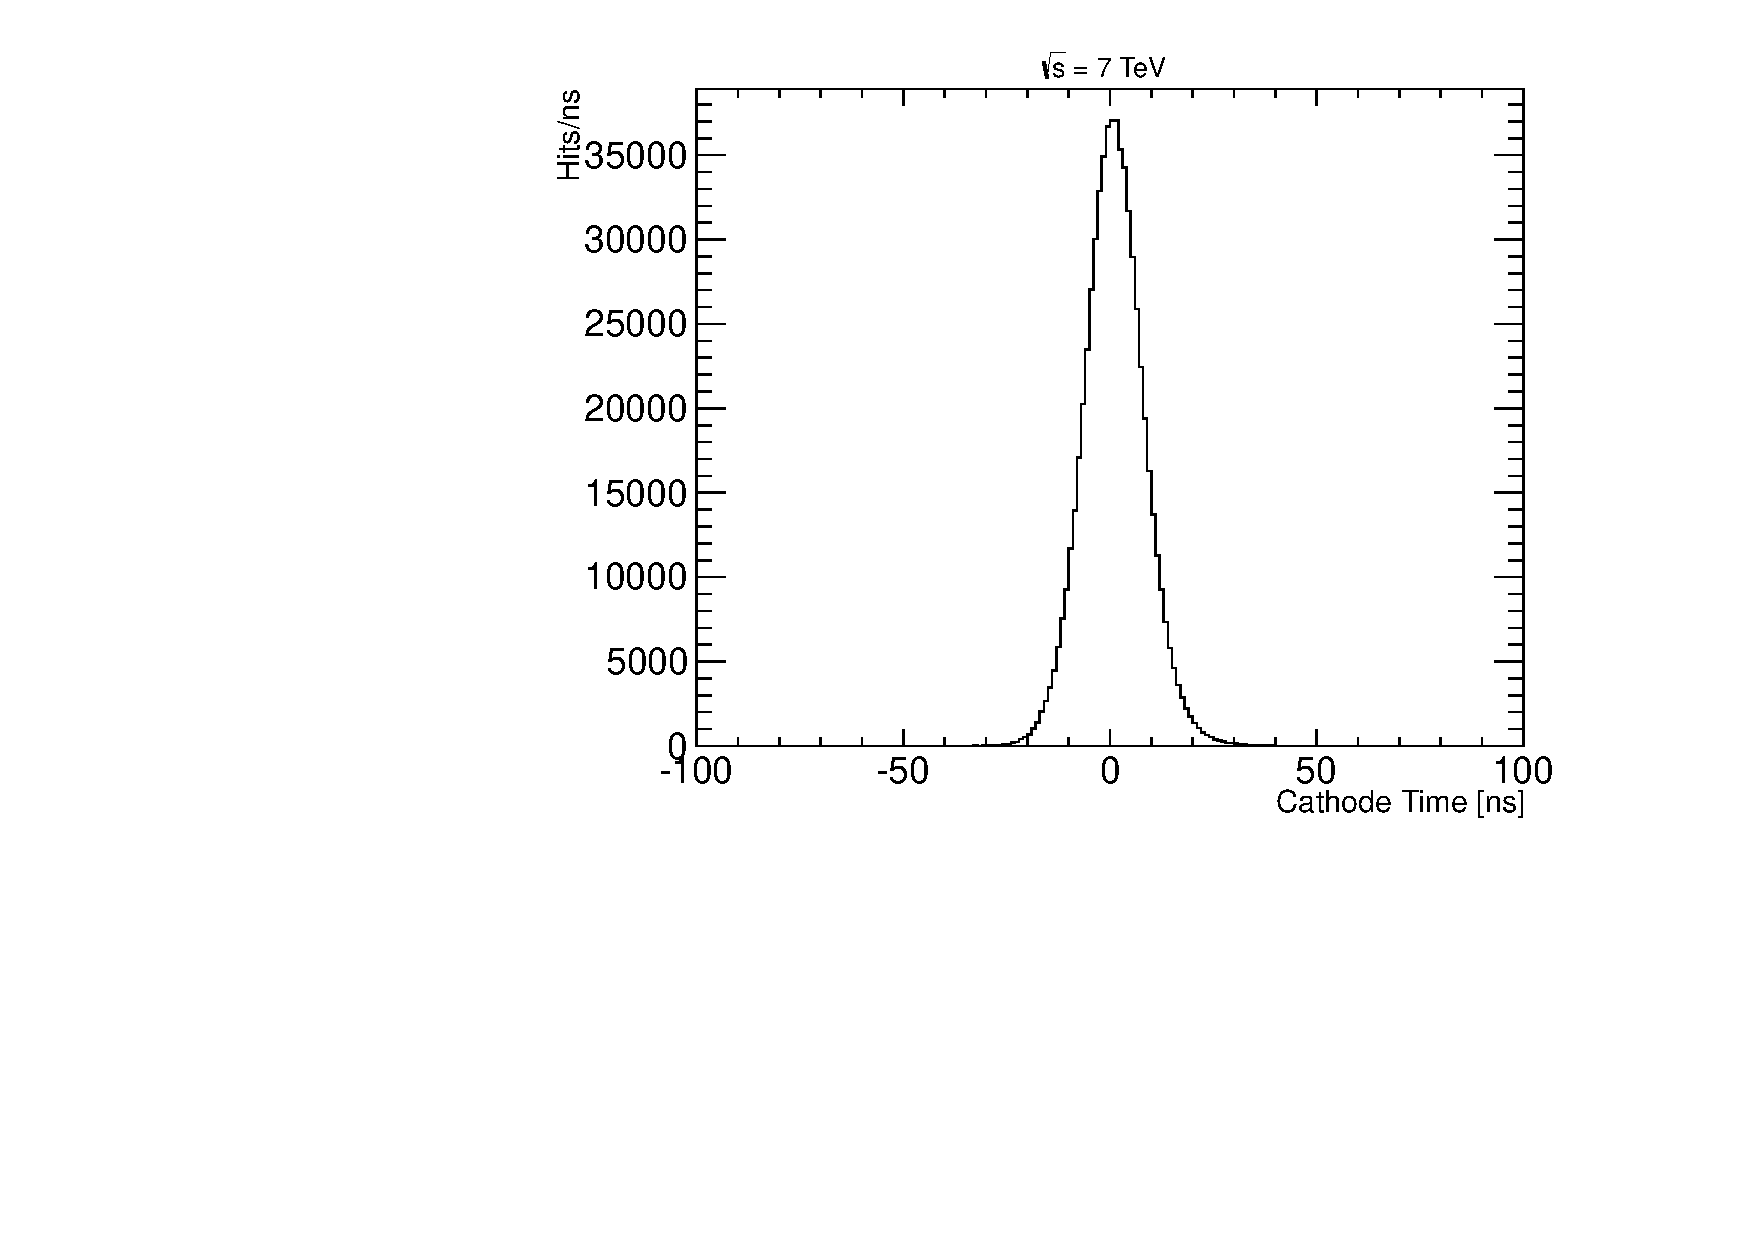
\includegraphics[clip=true, trim=0.0cm 0cm 0.0cm 0cm, width=0.48\textwidth]{figures/timing/CathodeTime}
      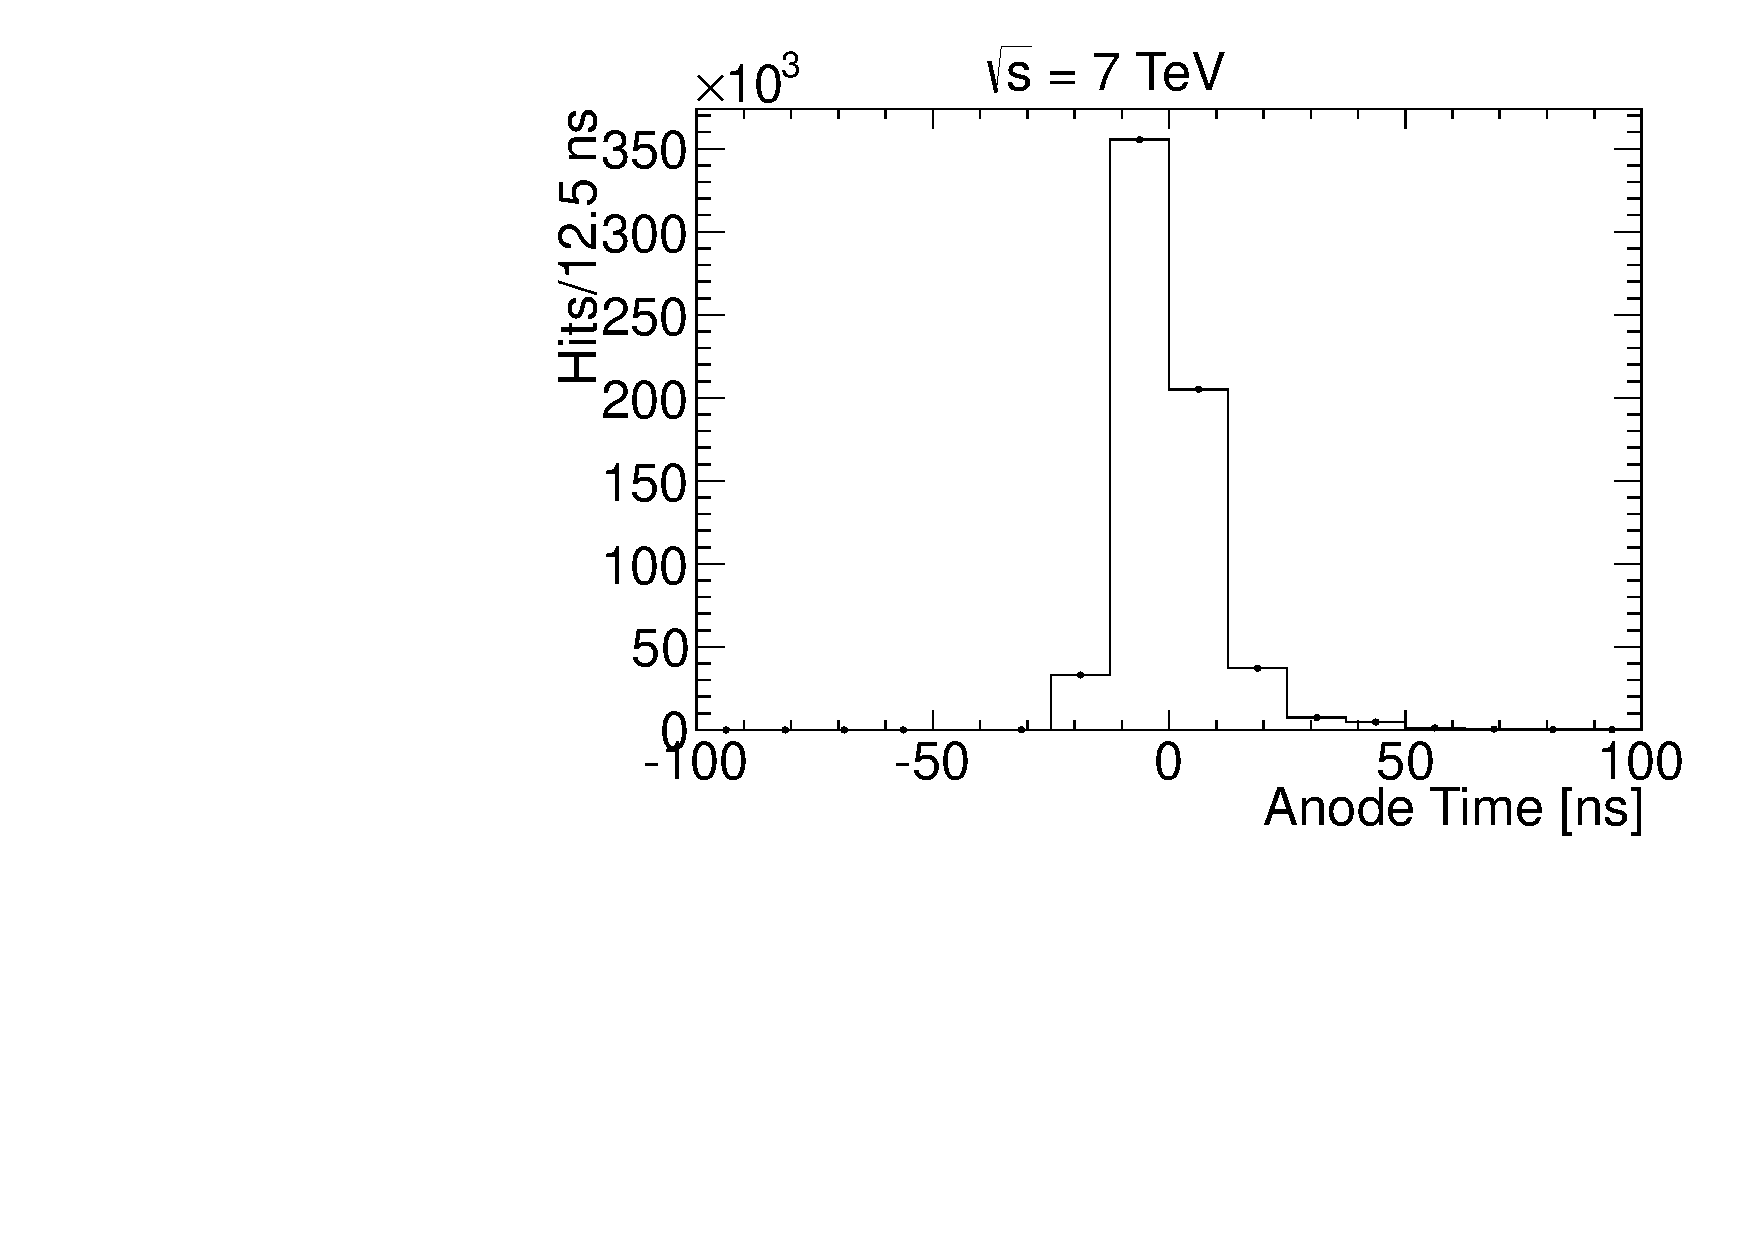
\includegraphics[clip=true, trim=0.0cm 0cm 0.0cm 0cm, width=0.48\textwidth]{figures/timing/AnodeTime} \\
      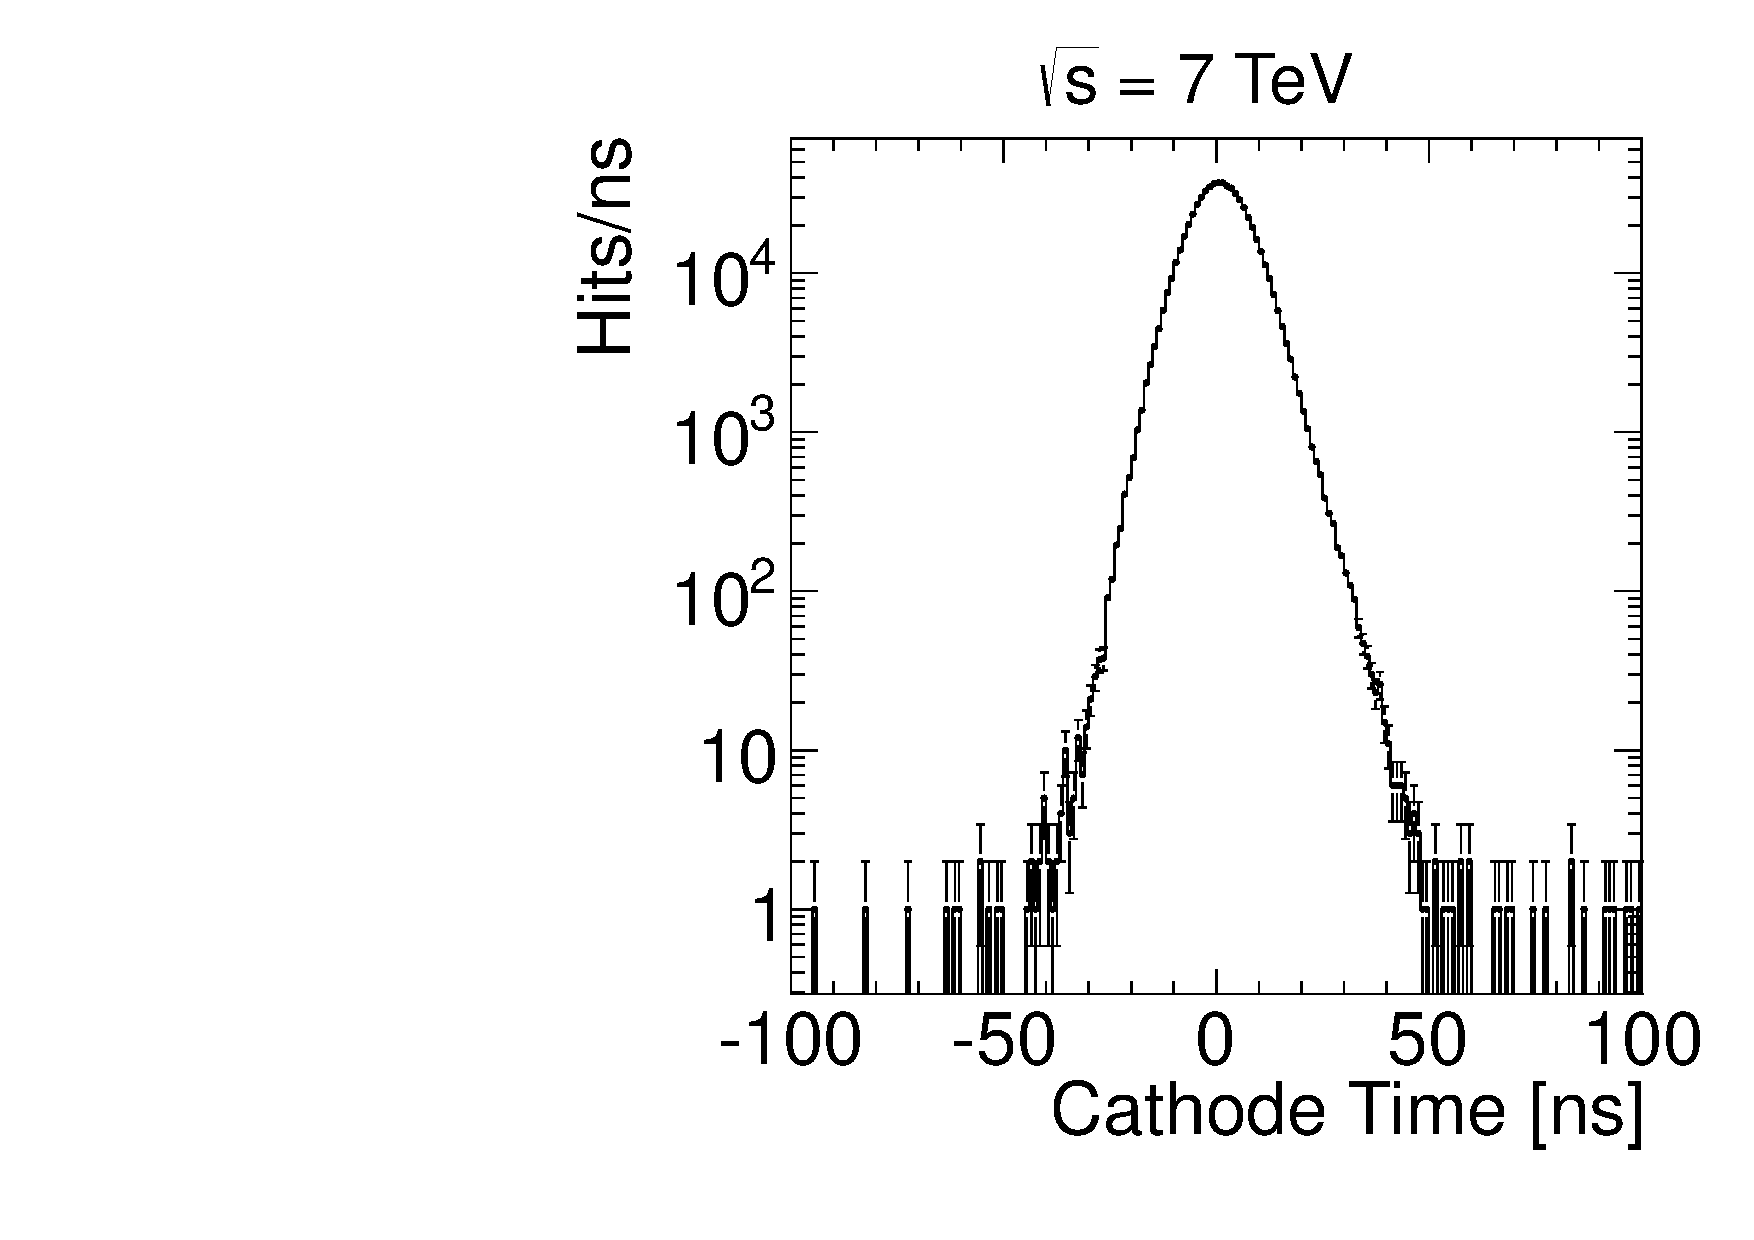
\includegraphics[clip=true, trim=0.0cm 0cm 0.0cm 0cm, width=0.48\textwidth]{figures/timing/CathodeTimeLog}
      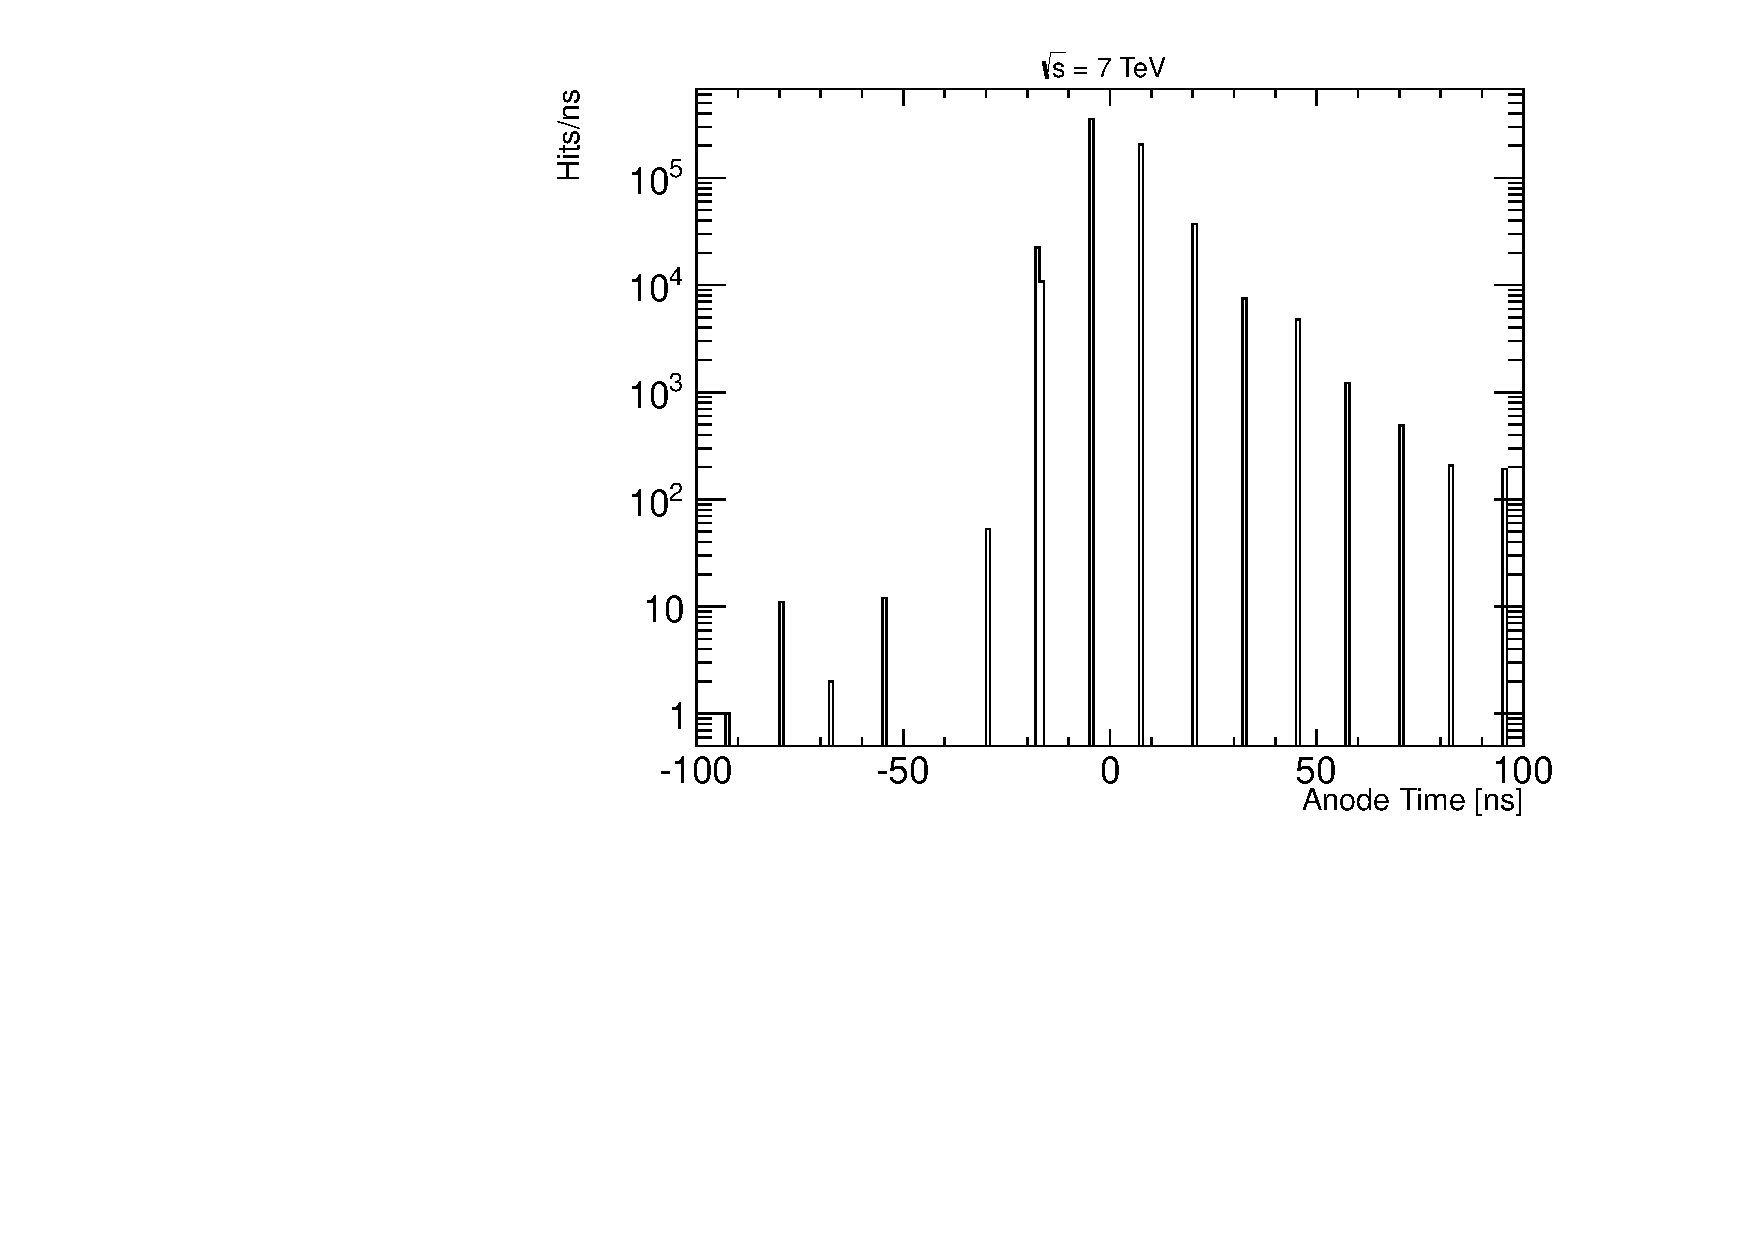
\includegraphics[clip=true, trim=0.0cm 0cm 0.0cm 0cm, width=0.48\textwidth]{figures/timing/AnodeTimeLog} \\
      \caption[Distribution of time of anode and cathode hits]
      {Distribution of time measured from cathode (left) and anode (right) hits.
The top row shows the times with a linear y-axis scale and the bottom is with log scale.
	}
      \label{fig:hittime}
  \end{center}
\end{figure}

The anode and cathode hits in a chamber are used to reconstruct a segment which is meant to represent the trajectory of the particle through the chamber. A time is
found for each segment by averaging the anode and cathode times associated with the segment. 
%The times are weighted by one over their variance.
%The variance is defined as the resolution of the measurement, 7~ns for cathode hits and 8.6~ns for cathode hits, squared.
To remove the large tail in the anode time measurement,
a cleaning procedure is applied to the anode times to remove outlier hits. The procedure calculates the average time of the segment and finds the anode hit with the largest
difference with the average. If the difference is larger than 26~ns, equal to three times the resolution,
that hit is removed from the average. The process is then repeated until the
anode hit with the largest difference is less than 26~ns.
The times of segments in data is shown in Fig.~\ref{fig:SegTimes}. 
The data sample used was collected at 7~TeV center--of--mass energy after the full commissioning of the timing measurement and has a \pt\ threshold of 20~GeV.
The resolution on the segment times is 3.0ns.

\begin{figure}
  \begin{center}
      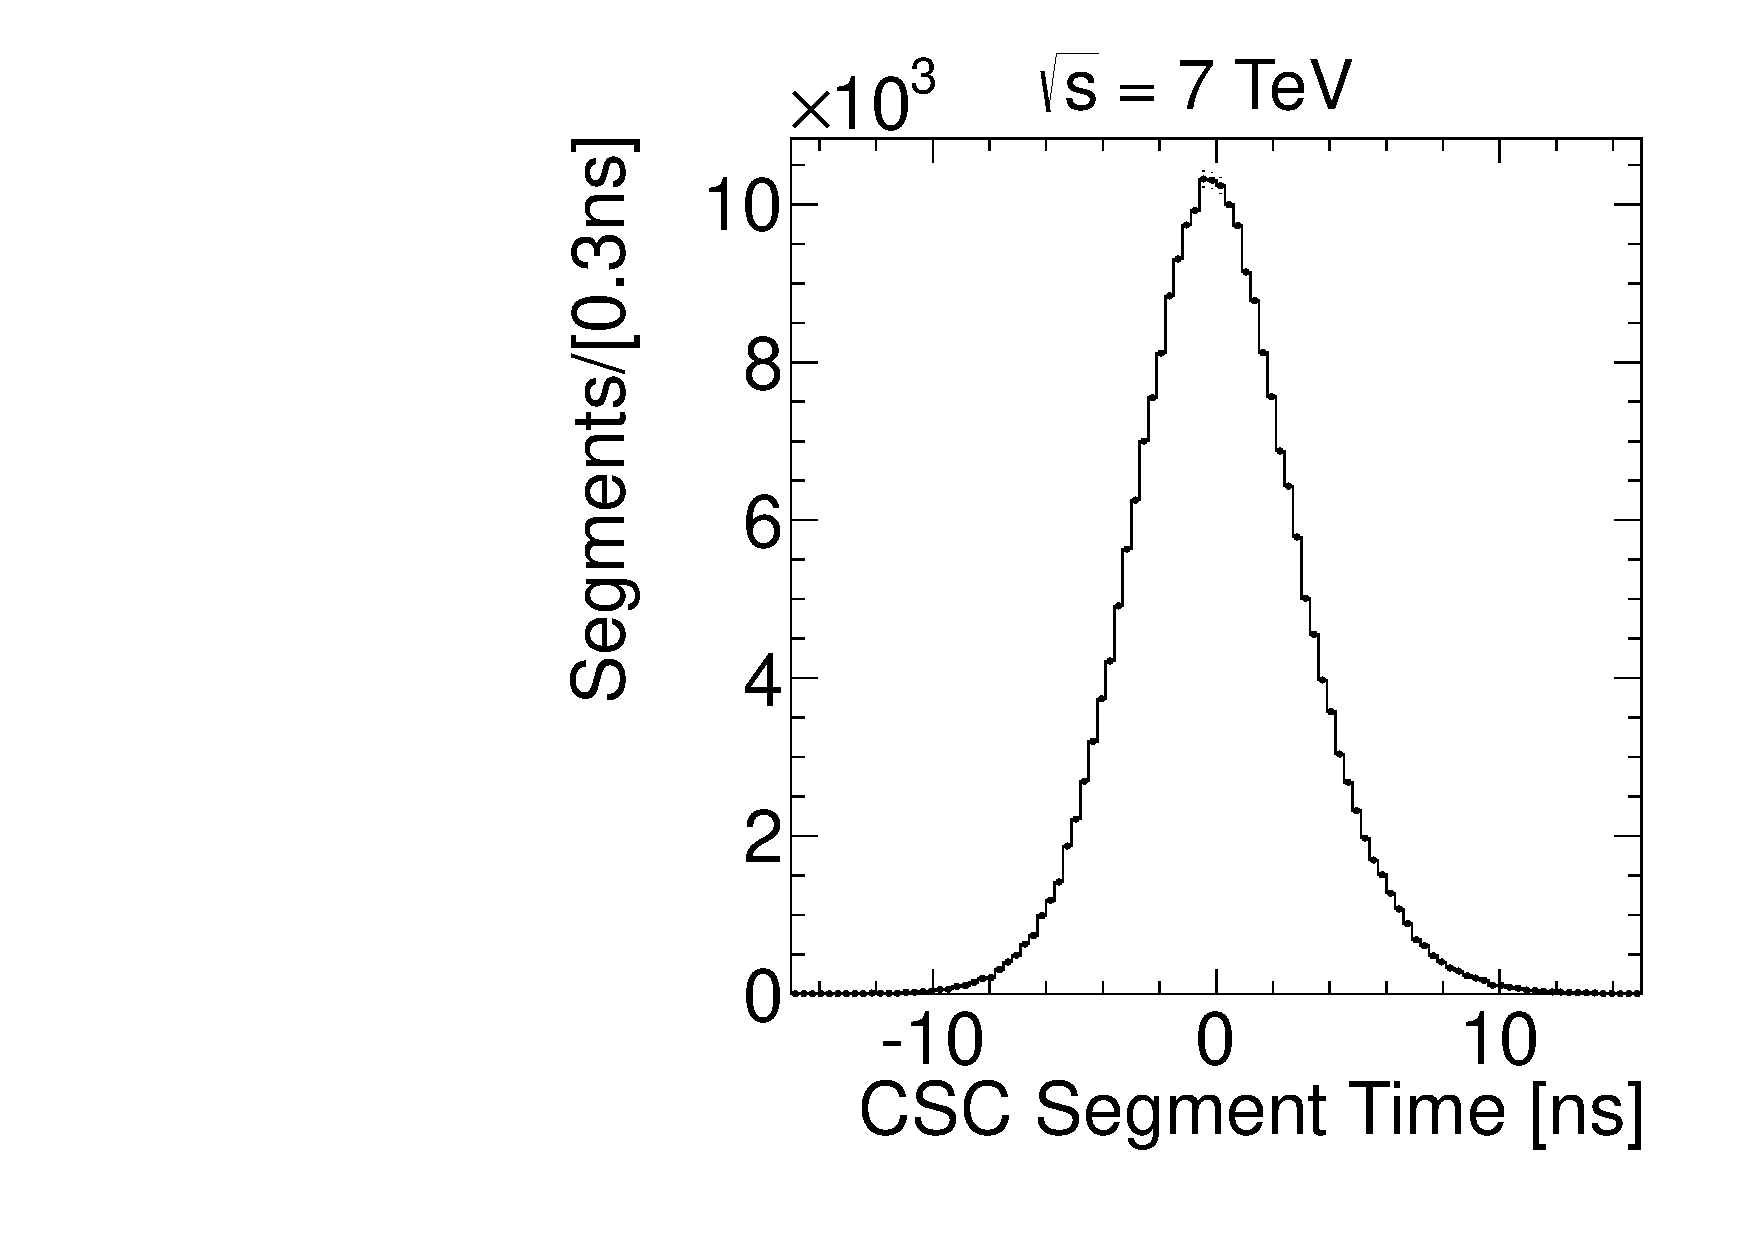
\includegraphics[width=0.44\textwidth]{figures/timing/StripAndWireSegmentTime}
      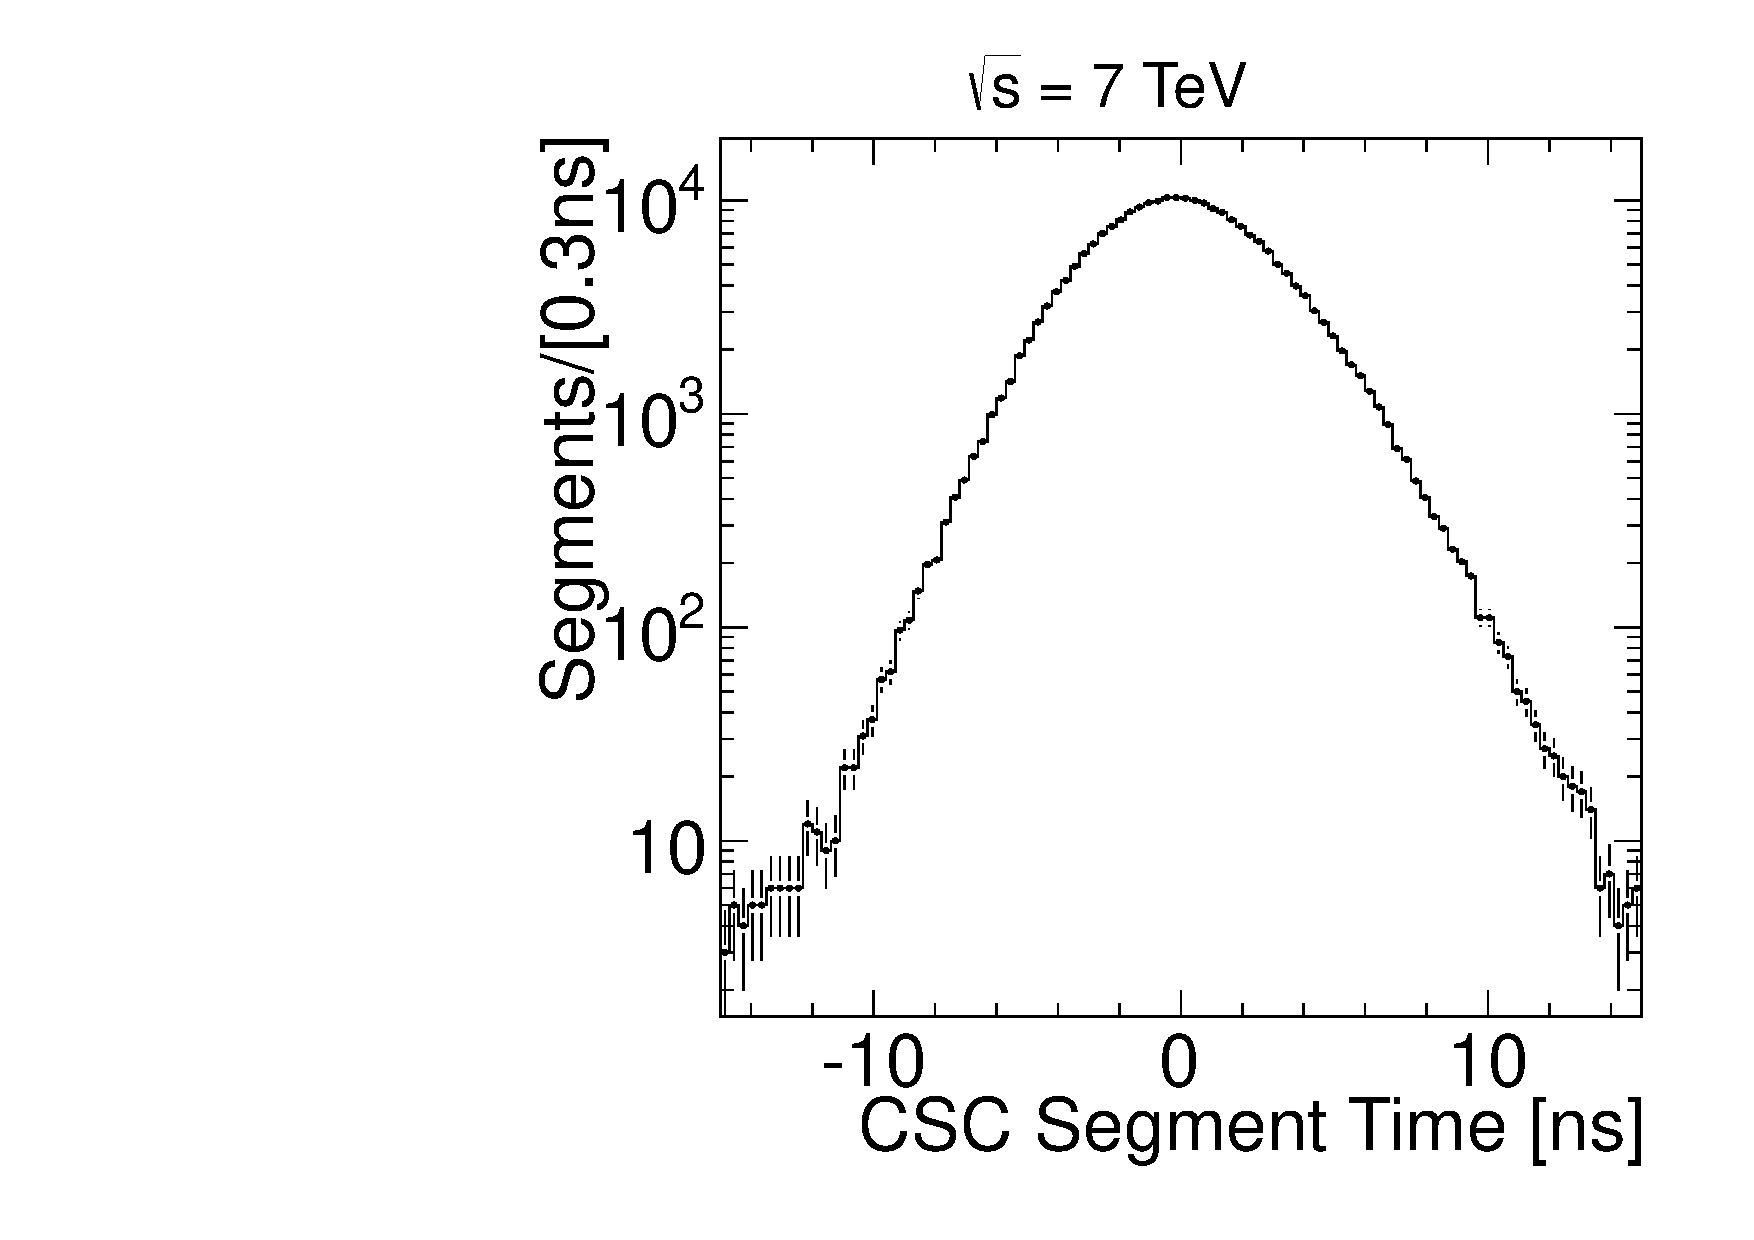
\includegraphics[width=0.44\textwidth]{figures/timing/StripAndWireSegmentTimeLog}
      \caption[Distribution of times of segments]
      {Times of segments associated with high-quality muons. Left with linear y-axis scale, right with log scale.
        }
      \label{fig:SegTimes}
  \end{center}
\end{figure}

\section{CSC Trigger Timing}

The CSCs are a key component of the L1 trigger system and it is important that they associate tracks in the system with the correct LHC bunch crossing window.
The CSCs build tracks for the L1 trigger with the CSC Track Finder (CSCTF)~\cite{2003physics...6117A} by combining track stubs coming from the CSC chambers. 
The stubs are associated with a particular bunch crossing window and
the CSCTF uses majority logic of the stubs used to build the track to associate the track with a bunch crossing window. In cases where there are an equal number
of stubs from different bunch crossing windows, say two track stubs coming from adjacent bunch crossing windows, the CSCTF preferentially selects the later bunch crossing window.

As mentioned in Section~\ref{sec:subsystems}, there are six layers of cathode strips and anode wires in a CSC chamber.
Electronics on the chamber collect hits from the cathode strips and anode wires and separately create trigger primitives called Cathode Local Charged Track (CLCT)
and Anode Local Charged Track (ALCT), respectively. The two separate trigger primitives are then combined to form a Local Charged Track (LCT). The ALCT and CLCT trigger primitives
must be associated with events within three bunch crossing windows of one another to be combined.
The bunch crossing window that the LCT is associated with is set by the ALCT.

The timing of the ALCT is determined by the timing of the third anode hit 
to arrive to the ALCT circuit board. A common offset per chamber can be applied to the
anode hits to give the best timing synchronization of the ALCTs. To determine the offset, the arrival time of the anode hits is studied offline. The average time of the anode
hits from a chamber can be correlated with the probability that the same chamber will produce an ALCT in the bunch crossing 
window before it should (pre-trigger) and after it should (post-trigger).
This can be seen in Fig~\ref{fig:AnodevsprePost} (left), which shows the probabilities for each chamber to pre-trigger and post-trigger as a function of the average
anode time of each chamber. The data used in the plot was collected in 2010 before the full commissioning of the trigger timing was complete.
The offsets for each chamber can be tuned to give an expected pre-trigger and post-trigger probability.
The chambers are split into three categories depending on which station and ring they belong to. One category is chambers in the
first ring and station, another the chambers in the first ring not in the first station, and the last those not in the first ring. The design of these chambers are all
slightly different so it is allowed for them to have different optimal times.

\begin{figure}
  \begin{center}
      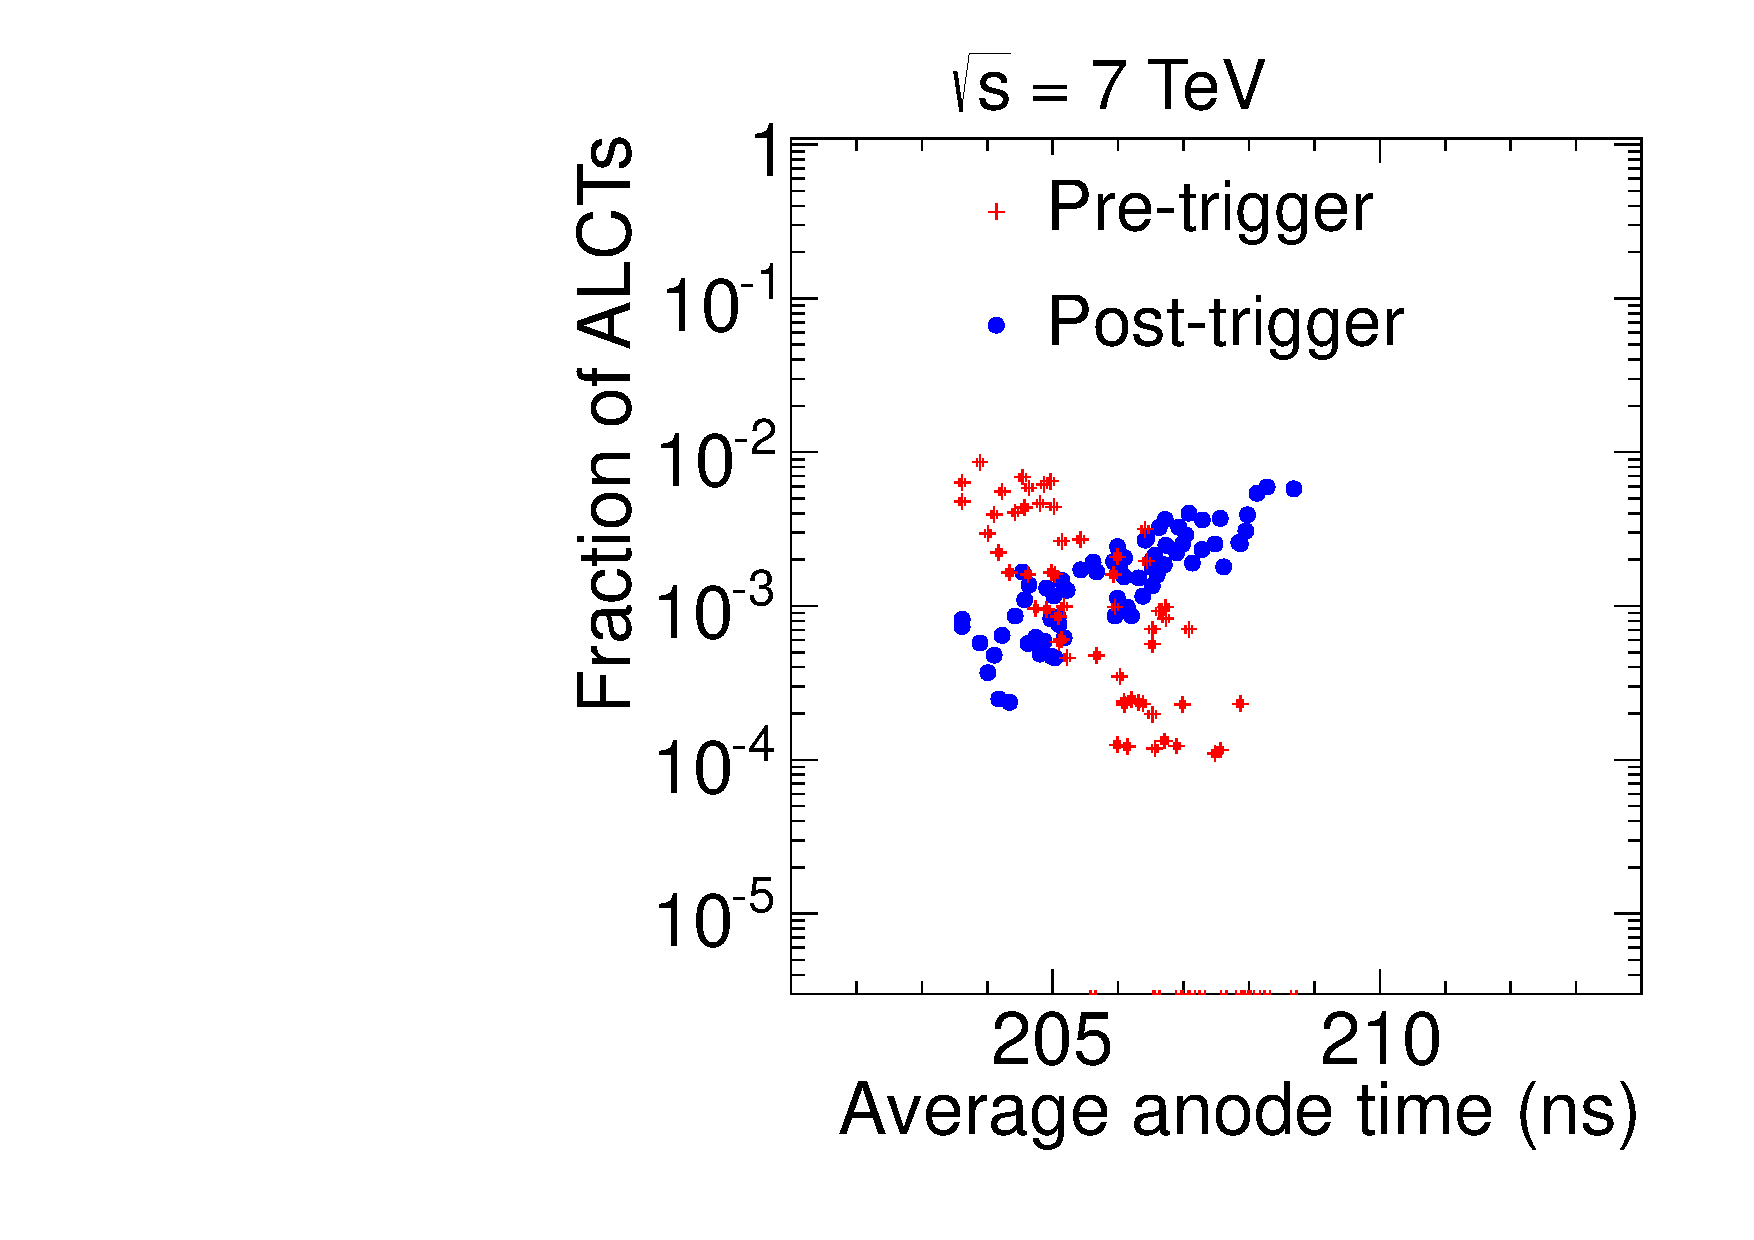
\includegraphics[clip=true, trim=0.0cm 0cm 0.0cm 0cm, width=0.44\textwidth]{figures/timing/ME11_Anode_vs_all3}
      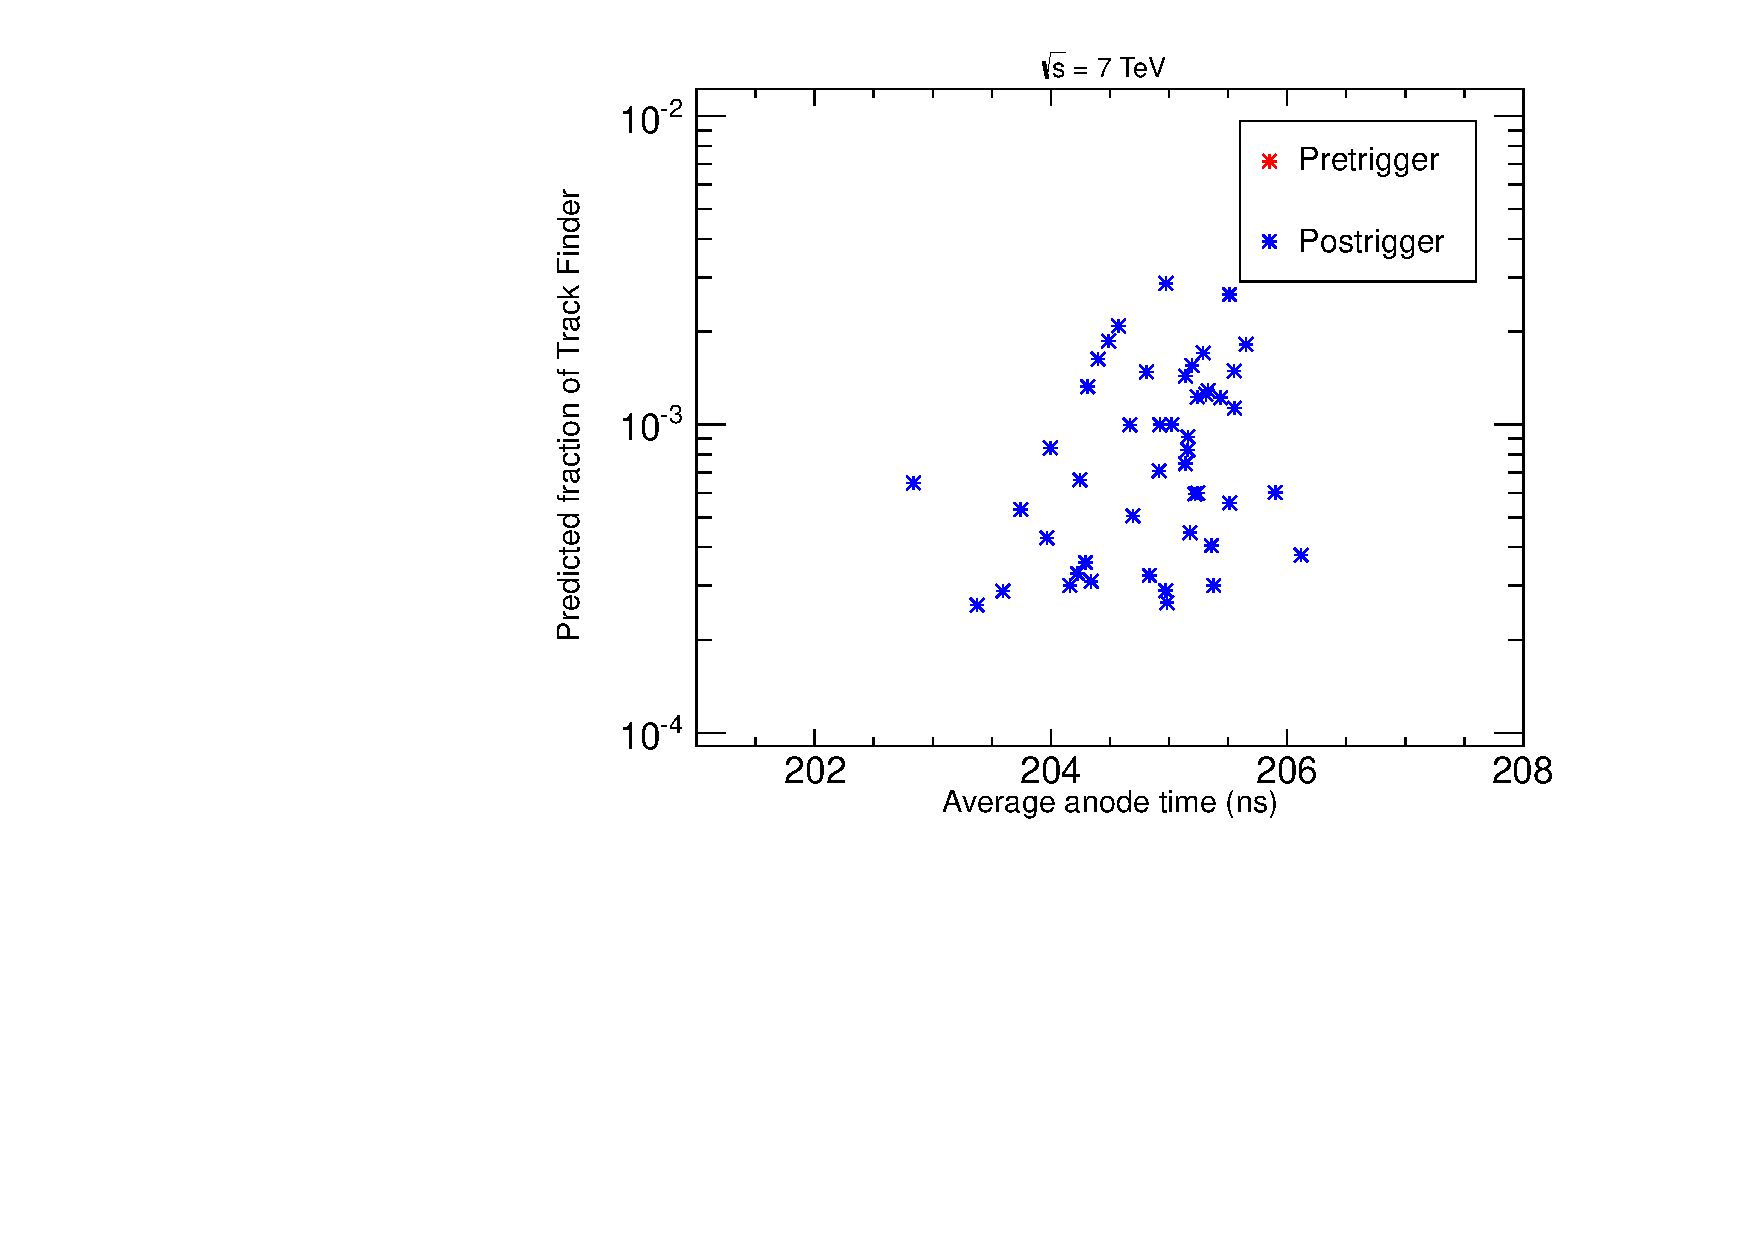
\includegraphics[clip=true, trim=0.0cm 0cm 0.0cm 0cm, width=0.44\textwidth]{figures/timing/ME11_Anode_vs_TF_all} \\
      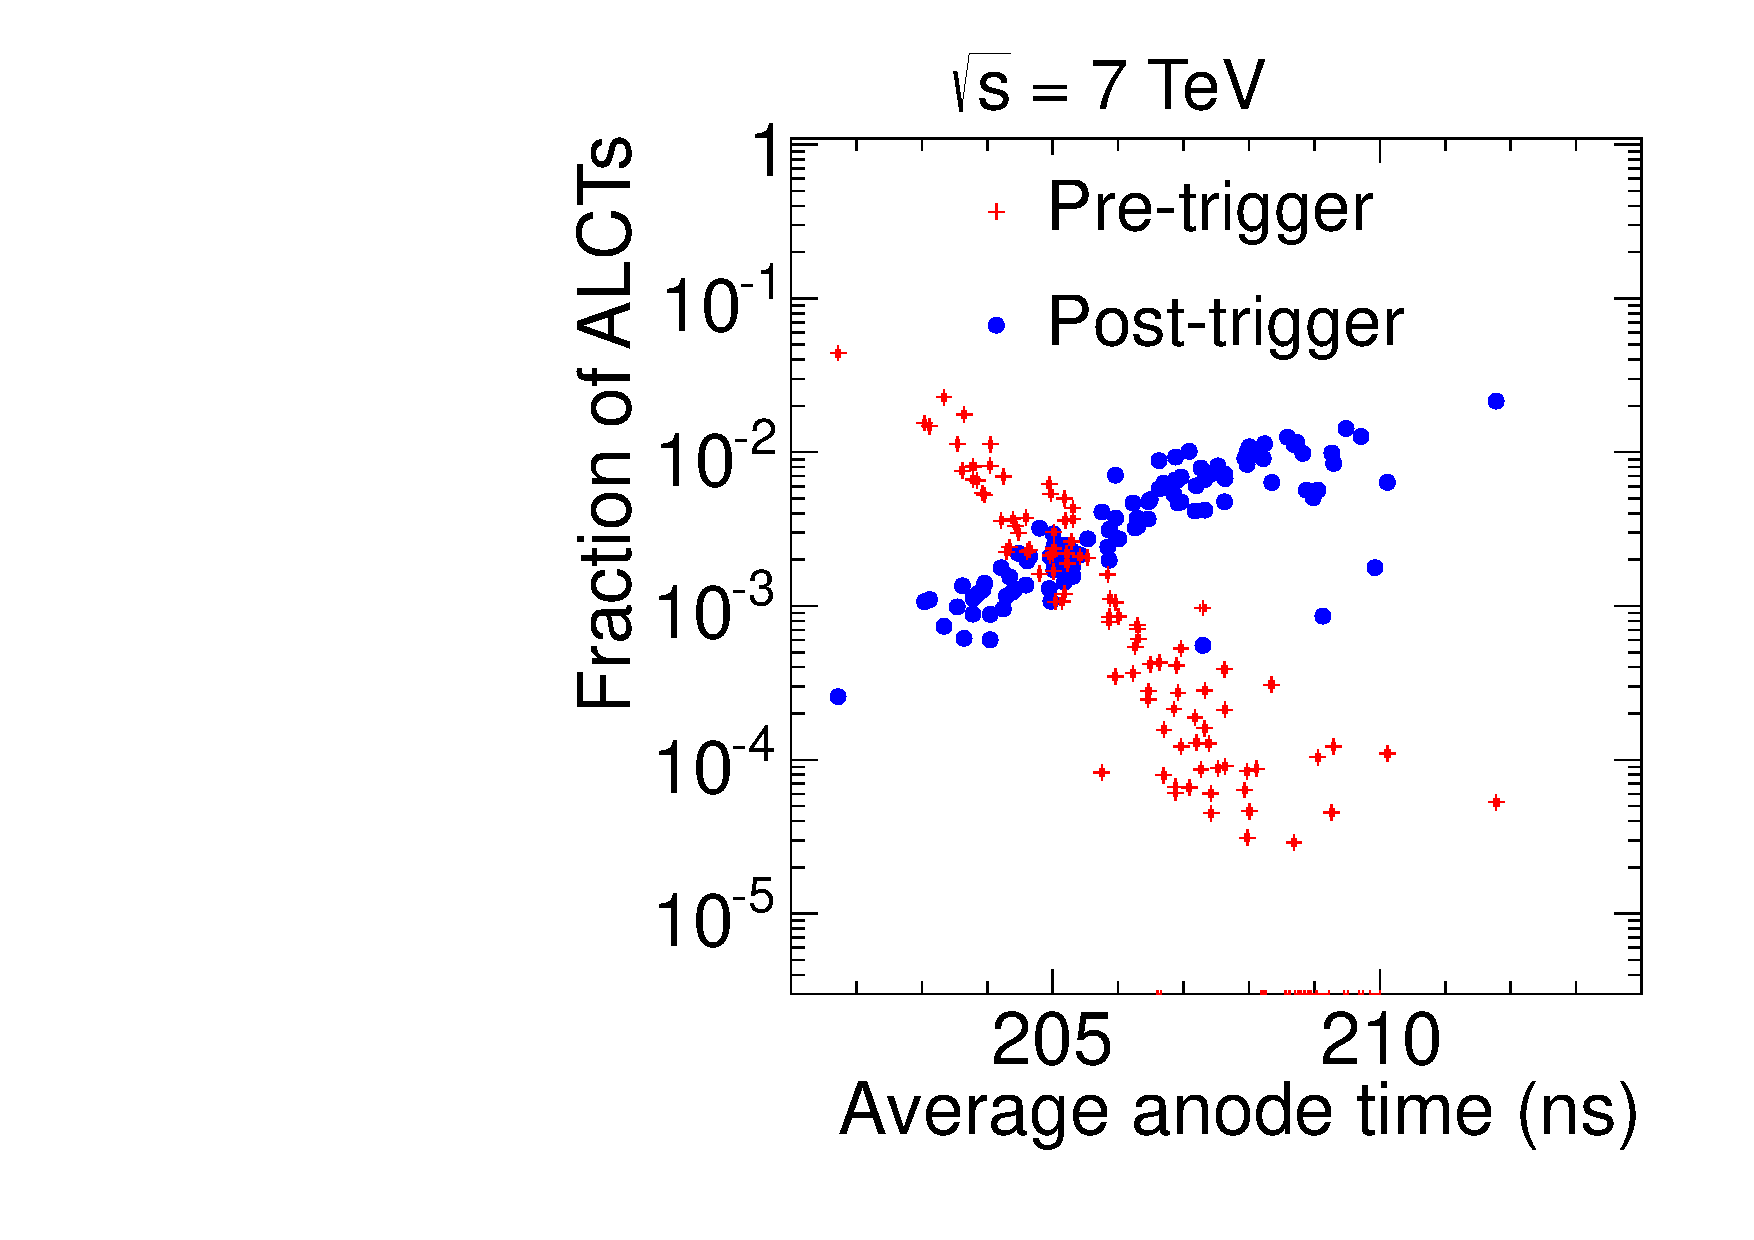
\includegraphics[clip=true, trim=0.0cm 0cm 0.0cm 0cm, width=0.44\textwidth]{figures/timing/Ring1_not11_Anode_vs_all3}
      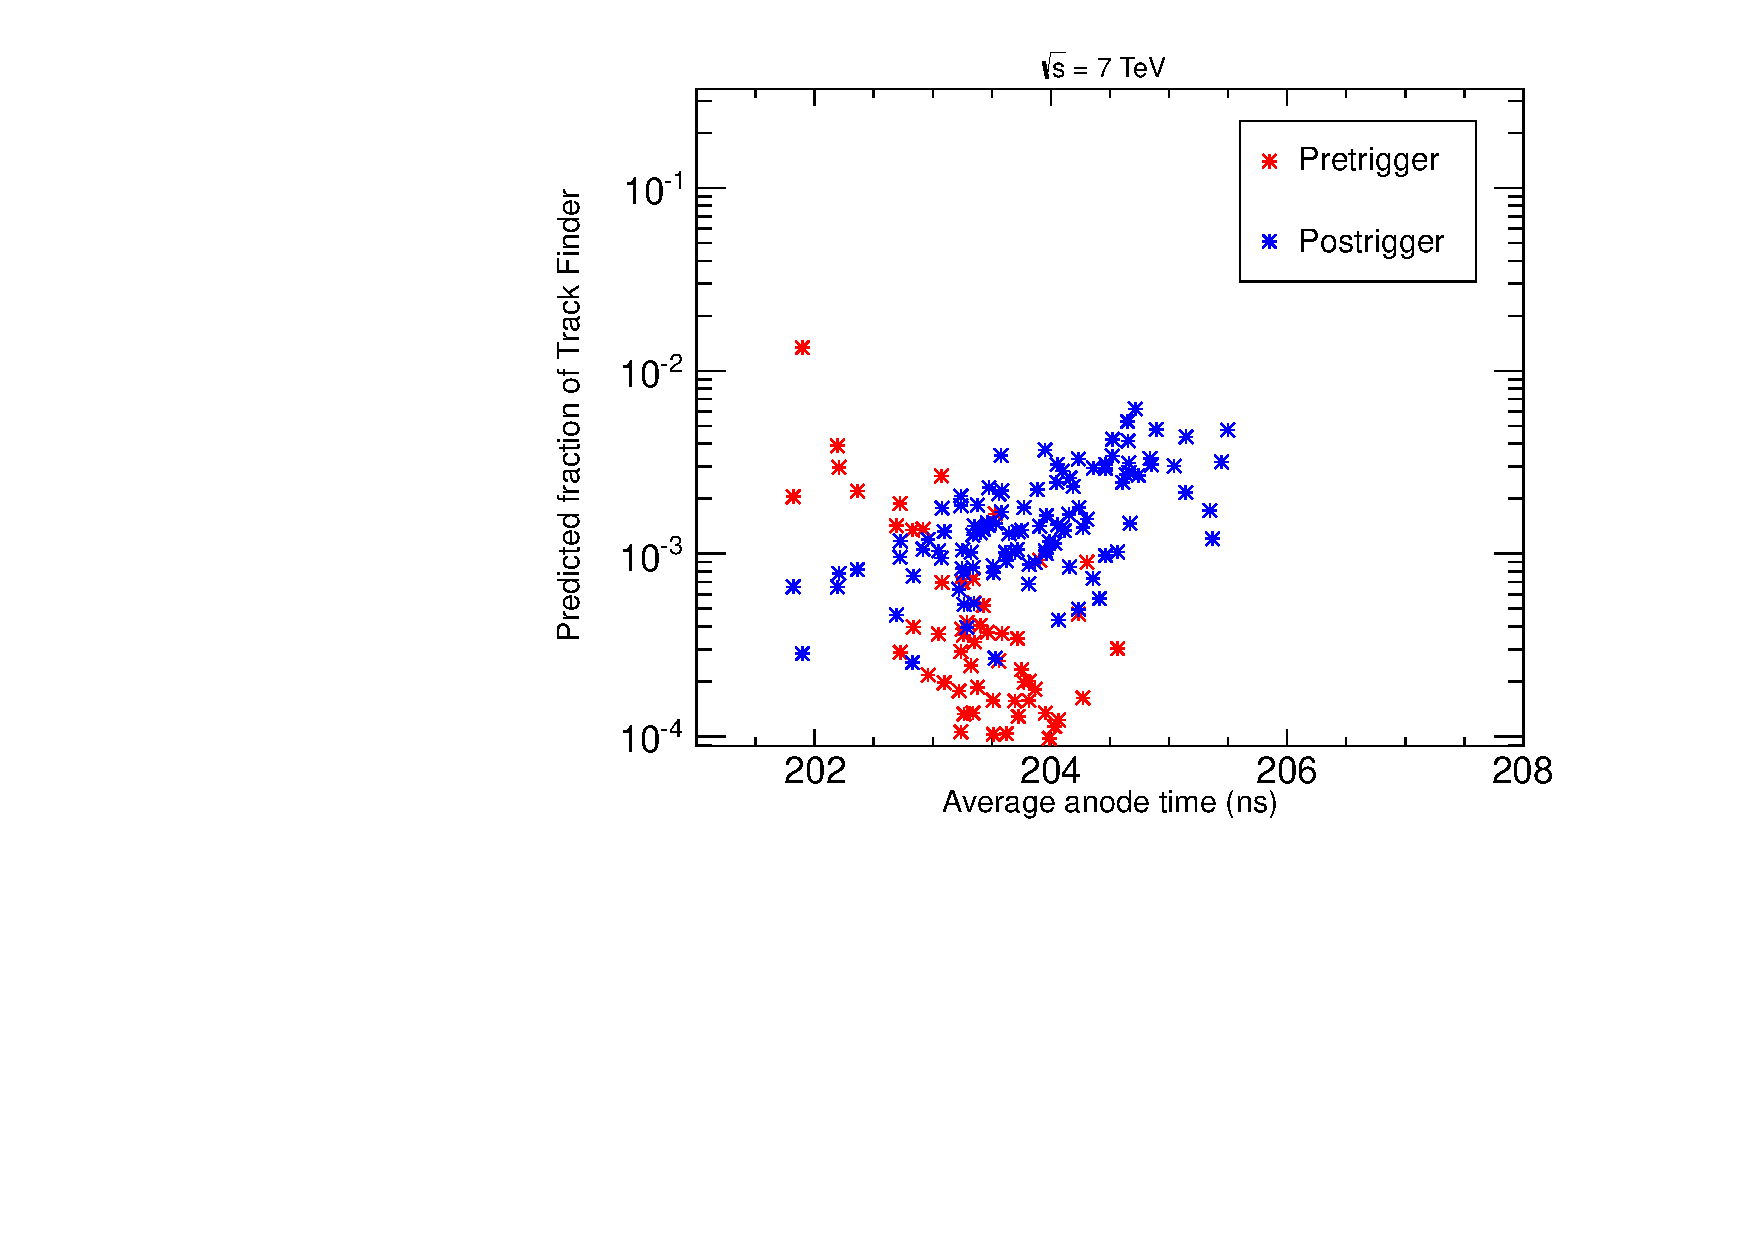
\includegraphics[clip=true, trim=0.0cm 0cm 0.0cm 0cm, width=0.44\textwidth]{figures/timing/Ring1_not11_Anode_vs_TF_all} \\
      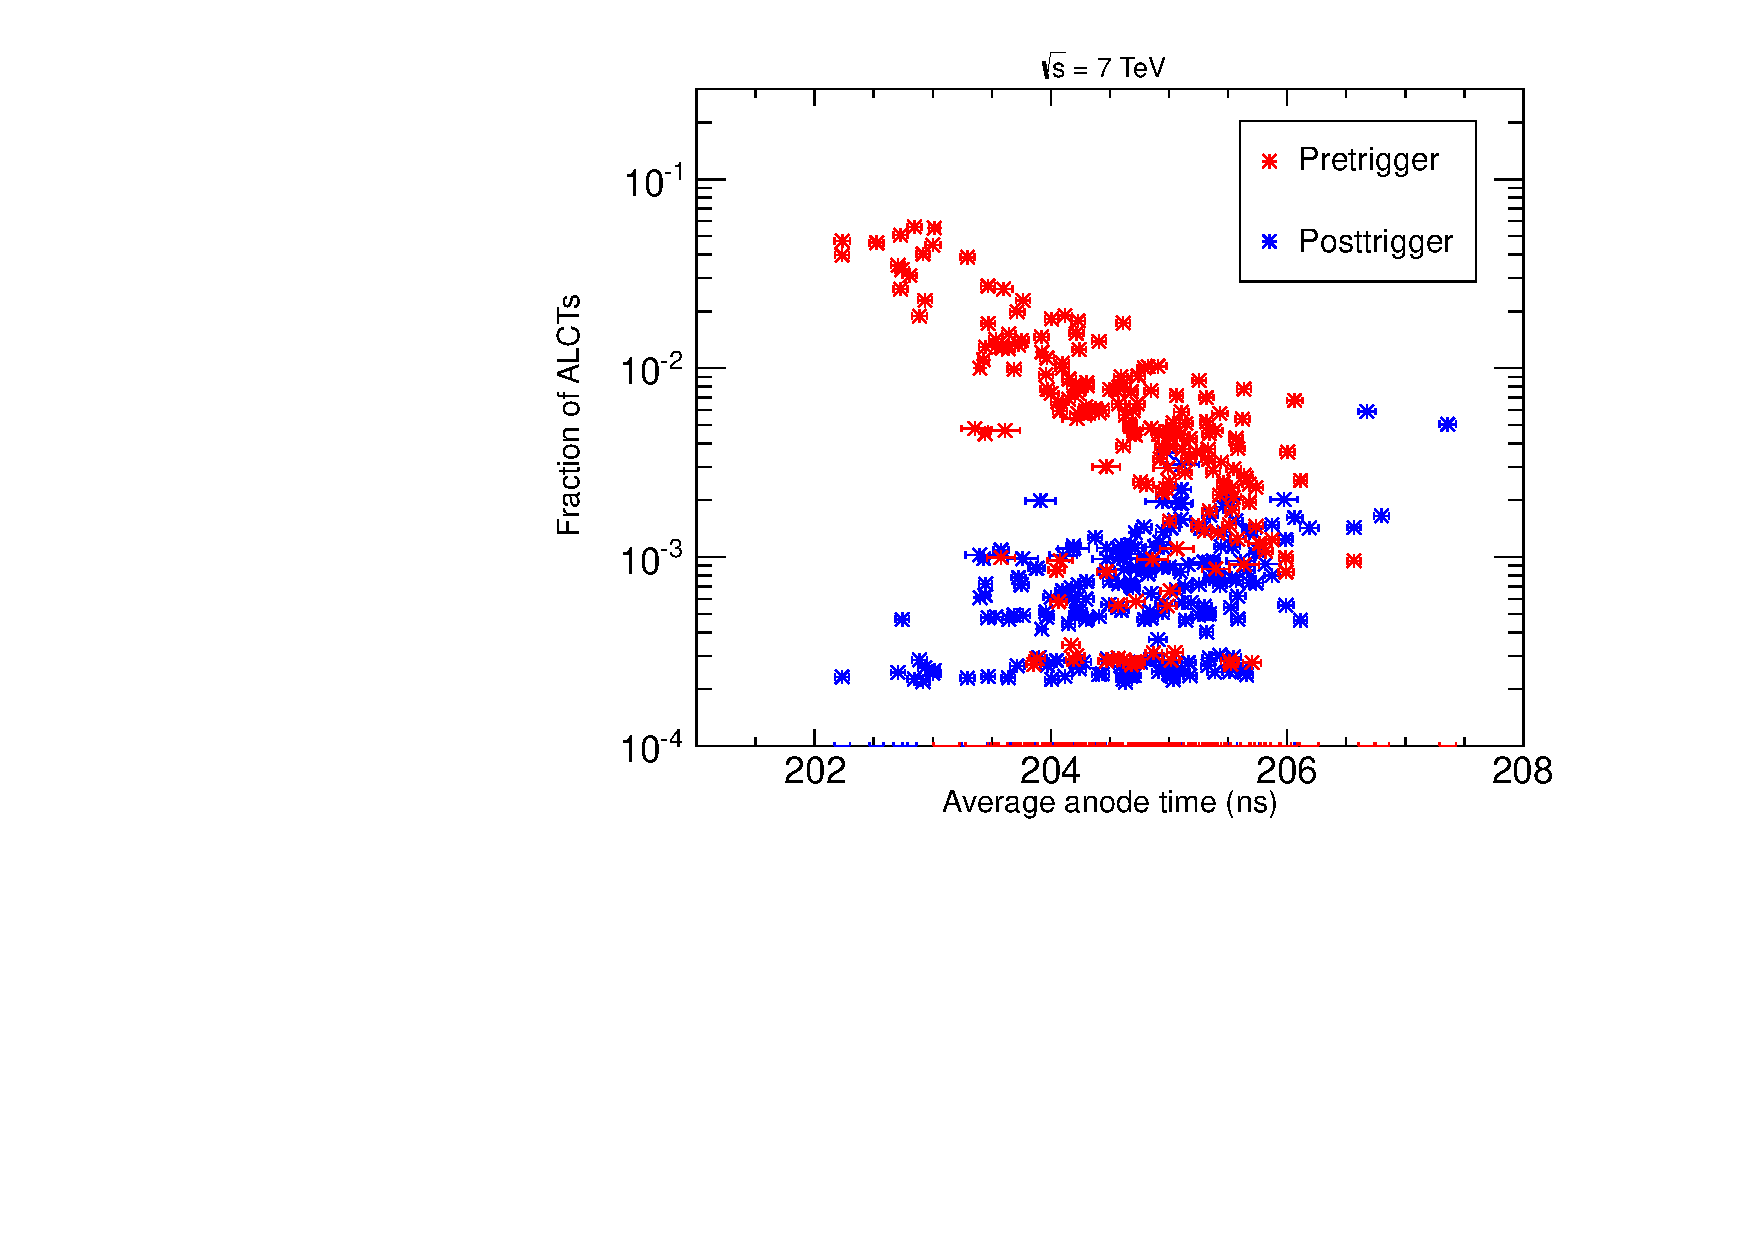
\includegraphics[clip=true, trim=0.0cm 0cm 0.0cm 0cm, width=0.44\textwidth]{figures/timing/Ring2_Anode_vs_all3}
      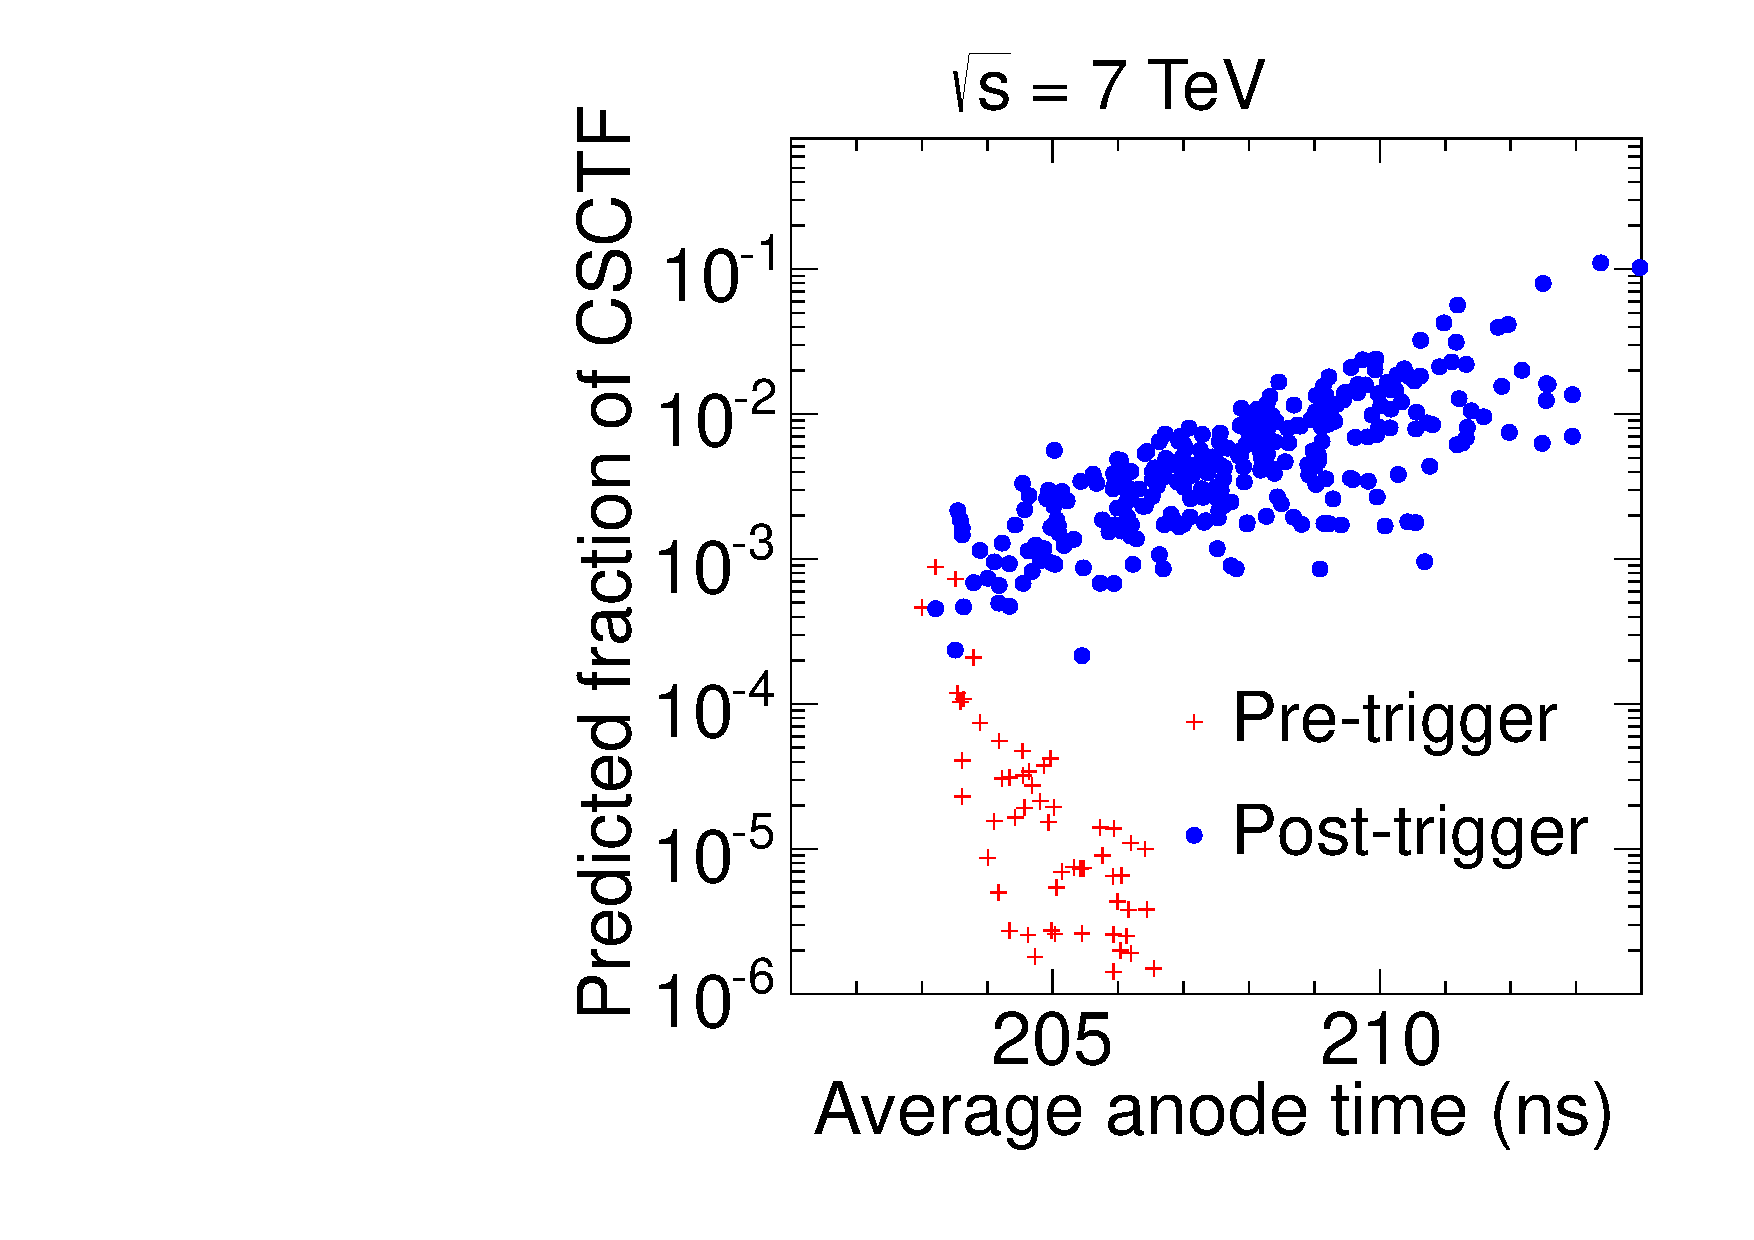
\includegraphics[clip=true, trim=0.0cm 0cm 0.0cm 0cm, width=0.44\textwidth]{figures/timing/Ring2_Anode_vs_TF_all} \\
      \caption[CSC pre-triggering and post-triggering versus average anode time for LCTs and expected behavior at CSCTF]
      {Pre-triggering and post-triggering probability versus average anode time. Left column shows the pre-triggering and post-triggering for LCTs.
Right column shows what would be expected at the CSCTF when only two track stubs are found.
Top row for chambers in the innermost ring and station. Middle row is for all other chambers in the innermost ring.
Last row is for all other chambers.
        }
      \label{fig:AnodevsprePost}
  \end{center}
\end{figure}

However, the CSCTF logic means that simply setting the offset to give an equal probability to pre-trigger and post-trigger is not optimal. This can be seen by looking at
the case where the CSCTF only receives two track stubs; this is also the case where the CSCTF is most sensitive to the offset. If the CSCTF receives one LCT in the bunch
crossing window before the collision and one in the correct bunch crossing window, it will preferentially choose the later LCT and associate the combined track with the correct
bunch crossing window.  In order to pre-trigger the readout of the event, more than one LCT must arrive early.
On the other hand, if it receives one LCT in the correct bunch crossing window and one in the proceeding bunch crossing window, the track will be associated with the
bunch crossing window following the collision. Thus, the probability to pre-trigger the event can be written as $P_{-}^2$ while the post-trigger probability can be written as
$2 \times P_{+} - P_{+}^2$ where $P_{-}$ is the probability to pre-trigger and $P_{+}$ is the probability to post-trigger.
Figure~\ref{fig:AnodevsprePost} (right) shows the expected probability to pre-trigger and post-trigger at the CSCTF assuming it receives two track stubs versus
the average anode time of a chamber.

From these plots an optimal value of 204~ns is chosen for the chambers in the first ring not in the first station and 205~ns for all other chambers.
The plot of the pre-triggering and post-triggering at the CSCTF somewhat suggests earlier times would be better but these are not used for two reasons.
The first is that pre-triggering at the CSCTF grows as the square of the LCT pre-triggering probability and since, as described below, the offsets can not be set exactly, chambers
that are slightly below optimal could lead to significant pre-triggering in those chambers. Second, pre-triggering prevents the readout
of the collision event even if a different part of CMS finds a signature that would normally trigger the readout of the detector as
CMS can not readout two consecutive events. Post-triggering does not have this issue as the post-triggered signal would be the one that is blocked.
For these reasons slightly later times that still have very low post-triggering probability are used.

The offsets can be moved in roughly 2~ns steps in the chamber electronics with the actual number possibly being different chamber to chamber. Shifting the offsets is a
somewhat complicated procedure and carries the risk of accidentally shifting the timing of a chamber by a large amount. Thus, the offsets are changed only
when deemed necessary and iterations to get a perfect synchronization are minimized. The synchronization with respect to the optimal values for all chambers
is shown in Fig.~\ref{fig:average_anodes} in data taken in 2010 after the offsets had been adjusted.
Most of the chambers are within one ns of the optimal time with none more than three ns off.

\begin{figure}
  \begin{center}
      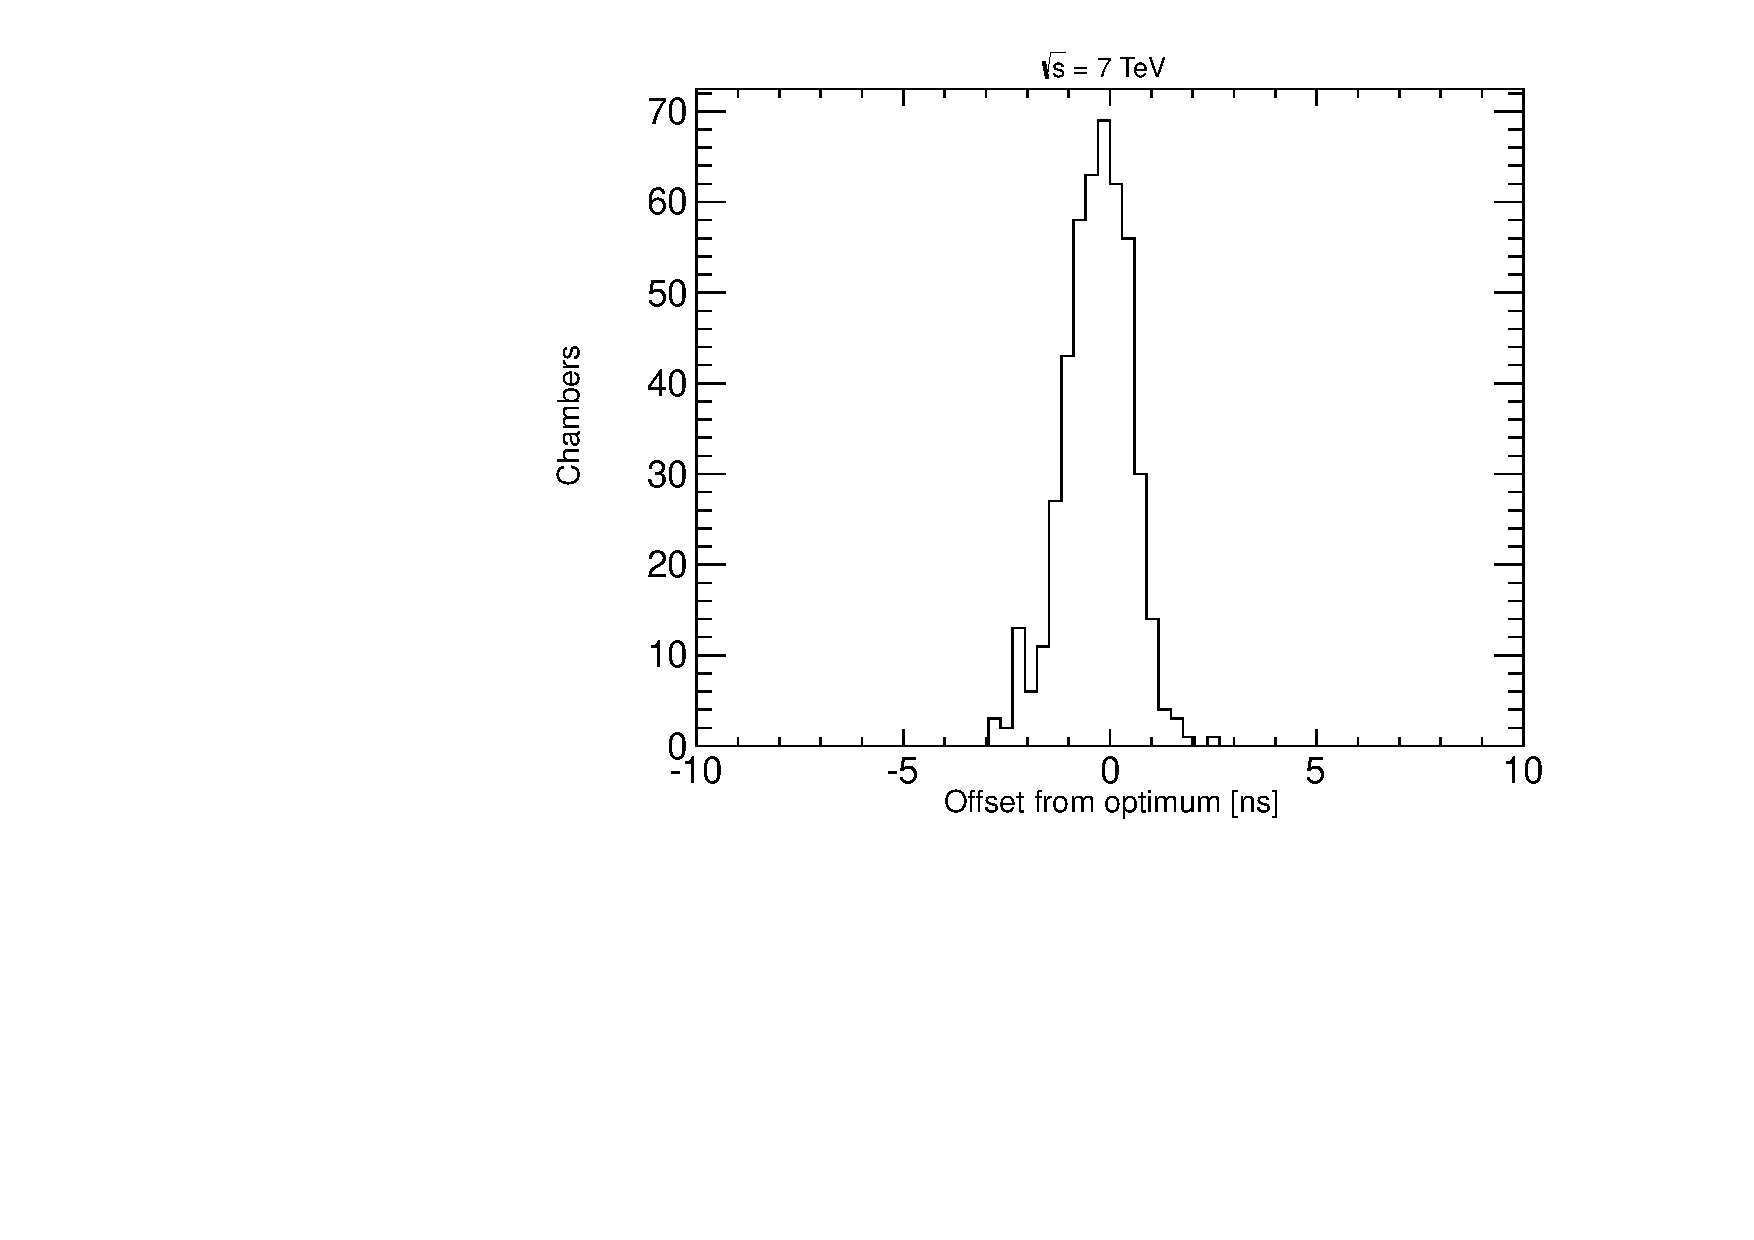
\includegraphics[clip=true, trim=0.0cm 0cm 0.0cm 0cm, width=0.44\textwidth]{figures/timing/average_anodes}
      \caption[Average anode time of chambers relative to optimal values.]
      {Average anode time of chambers relative to optimal values.
        }
      \label{fig:average_anodes}
  \end{center}
\end{figure}

After this synchronization procedure is performed the timing of the LCTs is very good. This can be seen in Fig.~\ref{fig:ALCTBX} which shows the bunch crossing window
assigned to LCTs matched to high-quality muons. The distribution is purposefully made asymmetric to account for the CSCTF logic used further downstream.
The efficiency to associate the LCT with the correct bunch crossing is 99\%, better than the 92\% design requirement from~\cite{Chatrchyan:2008zzk}.

\begin{figure}
  \begin{center}
      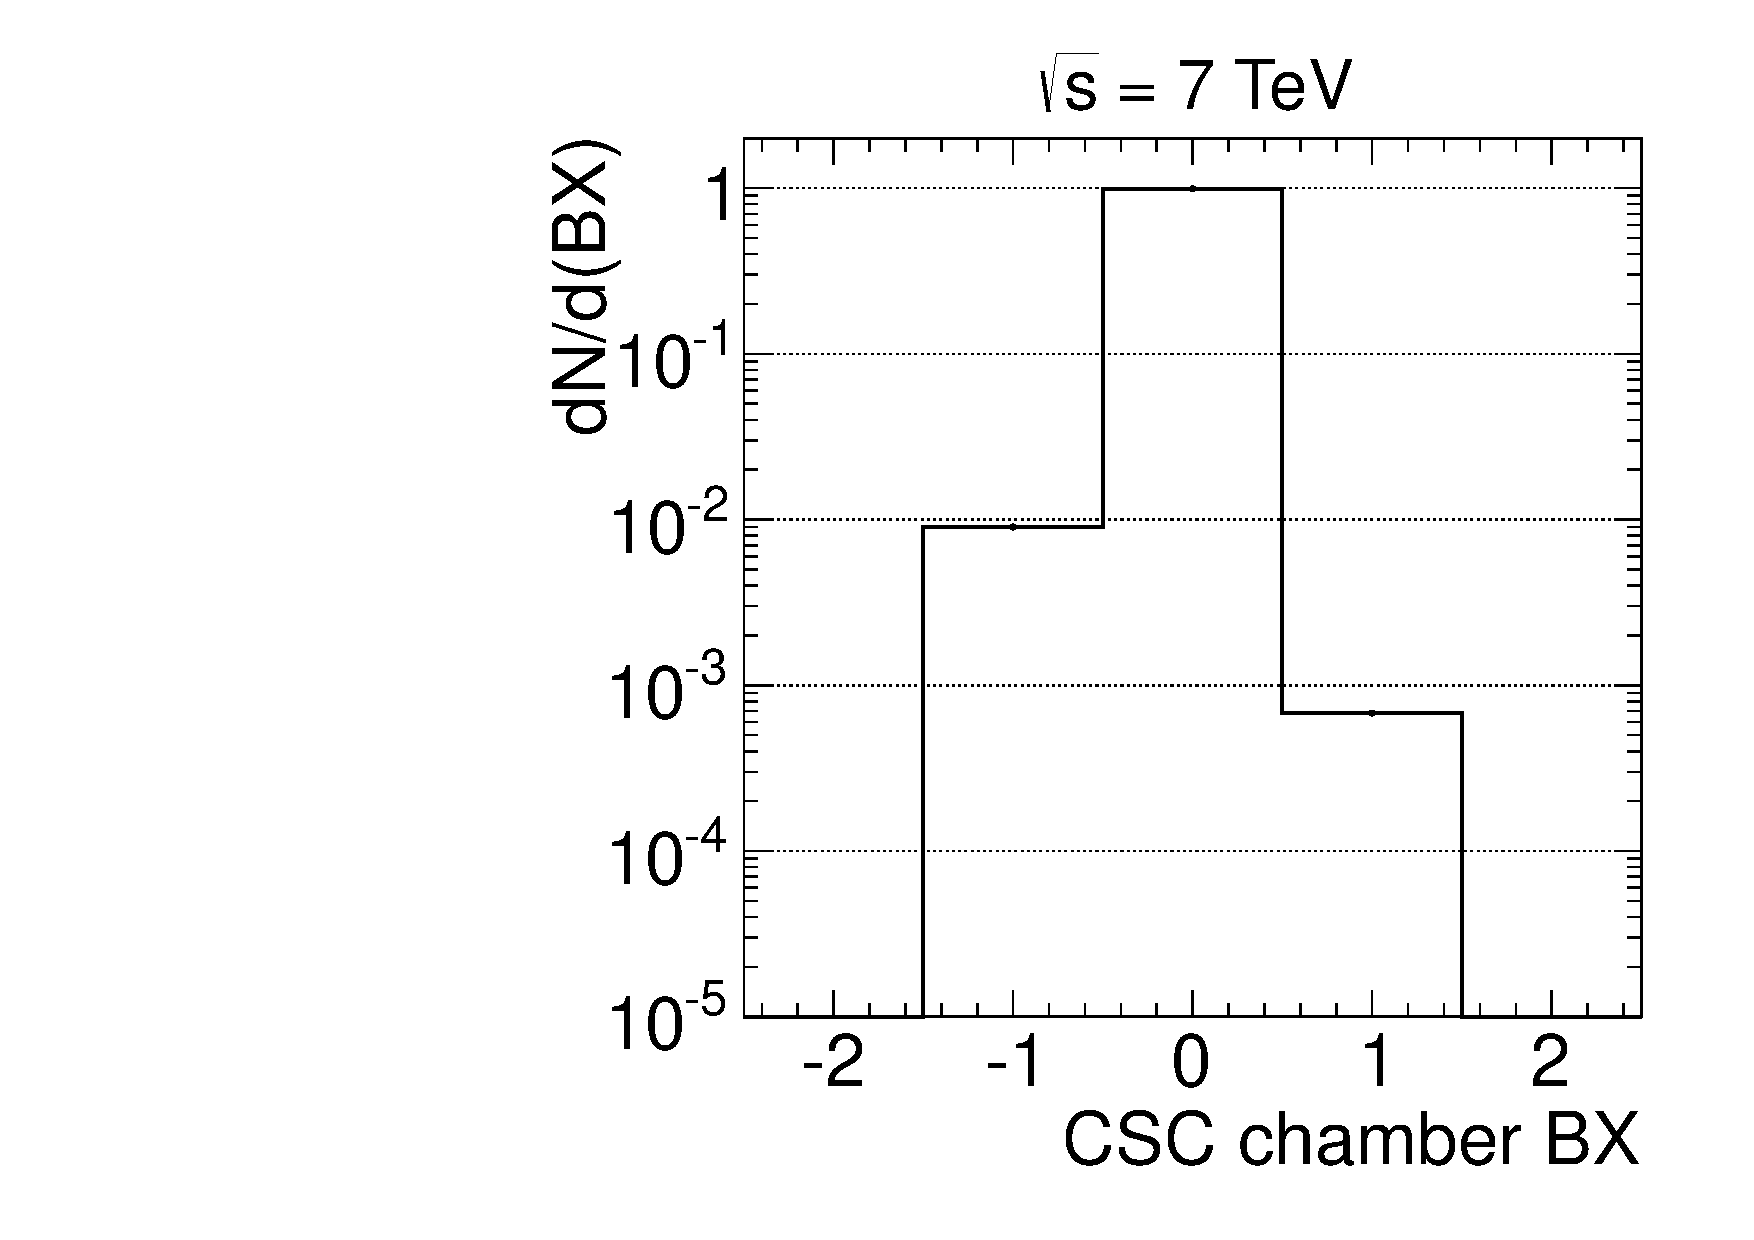
\includegraphics[clip=true, width=0.44\textwidth]{figures/timing/ALCT_Bx}
      \caption[Fraction of LCTs versus LCT bunch crossing window assignment relative to collision event]
      {Fraction of LCTs versus LCT bunch cross assignment relative to collision event
        }
      \label{fig:ALCTBX}
  \end{center}
\end{figure}

\section{DT Timing}

A complete description of the DT timing measurement can be found in~\cite{2007AN049}, a short summary is given here.
Tubes in consecutive layers of a DT chamber are staggered by half a tube, a particle will typical pass alternatively to the left and to the right of the
sensitive wires in consecutive layers.
The position of hits is inferred from the drift time of the ionization electrons assuming the hits come from a prompt muon.
For a late arriving HSCP, the delay will result in a longer drift time being attributed, so hits drifting
left will be to the right of their true position while hits drifting right will be to the left.
The DT time measurement then comes from the residuals of a straight line fit to the hits in the chamber.
The use of residuals means the uncertainty on DT time measurements decreases with more hits in a chamber as the trajectory of the particle in the
chamber becomes more well known. Only measurements from the $r-\phi$ superlayers are used in the time calculation as there are eight $r-\phi$ superlayers
per chamber while there are only four $r-z$ superlayers. Additionally, the measurements from the $r-\phi$ superlayers have been observed to be more uniform and precise than
those from the $r-z$ superlayers.

\section{Offline Muon Track Timing}

Tracks, meant to represent muons or other particles passing through the detector, are built in the muon system connecting together the hits in the different chambers of
the CSCs, DTs, and RPCs. The time measurements from the hits on the track can be used to estimate the speed of the particle and the time it left the interaction point.
Only time measurements from the CSCs and DTs are used to calculate the timing quantities.

A particle of speed $v$ traveling from the interaction point will arrive at a location $d$ in the muon system at
%~\ref{eq:speed}
\begin{equation}
t = d/v + t_0
\label{eq:speed}
\end{equation}
where $t_0$ is an overall offset. When the local timing variables were defined, they were calibrated such that a speed of light particle would have an average time
of zero. Thus $d/c$ has already been subtracted from the times so the same quantity must be subtracted from the right hand side of~\ref{eq:speed}.
Additionally it is easier to work with \invbeta\ ($\equiv{c/v}$) instead of $v$. With these two ideas taken into mind Eq.~\ref{eq:speed} now becomes
\begin{equation}
%\begin{split}
t = d/v - d/c + t_0 = (d / c) \times (\beta^{-1} - 1) + t_0 \\
%t &= d \times \beta^{-1} / c - d/c + t_0 \\
%t &= (d / c) \times (\beta^{-1} - 1) + t_0 \\
%\end{split}
\label{eq:speedred}
\end{equation}

Different assumptions can be taken on how the \invbeta\ and $t_0$ parameters are fixed, producing two different variables.
%The three assumptions relate to how the \invbeta\ and $t_0$ parameters are fixed and produce three different variables. 
The formula has two pieces of input datum: time and distance. The distance
from the interaction point to the hit location is known to a much better degree than the time of the hit so the uncertainty on the variables
is assumed to come entirely from the time measurement.

The first variable is the speed of the particle assuming it left the origin at $t_0 = 0$ reducing Eq.~\ref{eq:speedred} to 
$\beta^{-1} = tc/d + 1$. The measurement of \invbeta\ comes from the weighted average of this quantity for all the
CSC and DT hits associated with the track.
The weight $w$ for CSC measurements is
\begin{equation}
w = \left(\frac{d}{\sigma c}\right)^2
 \label{betaweight}
\end{equation}
where $d$ is the distance from the hit location to the interaction point
and $\sigma$ is the time resolution of the hit, 7.0~ns for cathode measurements and 8.6~ns for anode measurements as described above.
The weight for DT measurements is 
\begin{equation}
 w = \frac{(n-2)}{n}\left(\frac{d}{\sigma c}\right)^2
\end{equation}
where $n$ is the number of $\phi$ projection measurements found in the
chamber from which the measurement comes and the resolution $\sigma$ is three~ns.
The factor ${(n-2)/n}$ accounts for the fact that residuals are computed
using two parameters of a straight line determined from the same
$n$ measurements (the minimum number of hits in a DT chamber
needed for a residual calculation is $n=3$).
% in the same manner as was done to caluclate their segment times.
Outlier times from anode hits are again cleaned in the same manner as per the segment times. 
%The weighting by one over variance and outlier cleaning is performed for all three measurements.

The motivation for using \invbeta\ now becomes clear; the \invbeta\ measurement
is linear with t, the source of its uncertainty. This means that \invbeta\ will have a much more normal shape than $\beta$ which would be skewed.
An important point here is that the distribution will be close to symmetrical for near speed-of-light muons coming from the LHC.

The uncertainty on \invbeta\ can be calculated according to the formula
\begin{equation}
 \sigma_{1/\beta} = \sqrt{\sum_{i=1}^N \frac{(1/\beta_i - \overline{1/\beta})^2 \times w_{i}}{N-1}},
 \label{betaerr}
\end{equation}
where $\overline{1/\beta}$ is the average \invbeta\ of the track, $w_{i}$ is the weight of the $i^{th}$ hit, and N is the number of measurements associated with the track.

The speed of the particle is very useful in separating SM muons from HSCP produced in new physics as is shown in Chapter~\ref{sec:search}.
Figure~\ref{fig:invbeta} shows the \invbeta\ measurement, its uncertainty, and the number of degrees of freedom (d.o.f.) for the measurement for:
data collected in 2012 at 8~TeV, dominated by collision muons; 
muons from the simulated Drell-Yan production of Z bosons and photons at 8~TeV; cosmic-ray muons, the sample is defined in Section~\ref{sec:samples};
and HSCPs, again the sample is defined in Section~\ref{sec:samples}. All of the samples are required to pass the tight requirements on track quality
as defined by the Muon POG except for the cosmic-ray muon sample for which the only requirement is that the track be reconstructed in the muon system.
It can be seen that the \invbeta\ measurement for data and SM MC are strongly peaked at one, the cosmic-ray muons are roughly flat, while
the HSCP have \invbeta\ greater than one, indicating they are traveling slowly. The \invbeta\ measurement is slightly asymmetric about one for data and SM MC
due to the production of delta rays in the muon system which result in early timing measurements in the DTs. The shape of the distribution for cosmic-ray muons
is caused by them passing through both the top and bottom halves of CMS and possibly having tracks be reconstructed in both halves.
The timing of hits from the two tracks will be separated by approximately 40--80~ns.
One of the tracks will trigger the readout of CMS and thus will have \invbeta\ roughly around one, these tracks form the plateau in the cosmic-ray muon \invbeta\
distribution between zero and two. If the other track is also reconstructed its hits will have timing before zero, if the bottom track triggered the readout of CMS, or
after zero, if the top track triggered the readout of CMS. These two possibilities cause the adjacent plateaus at low and high \invbeta\ values.

\begin{figure}
  \begin{center}
      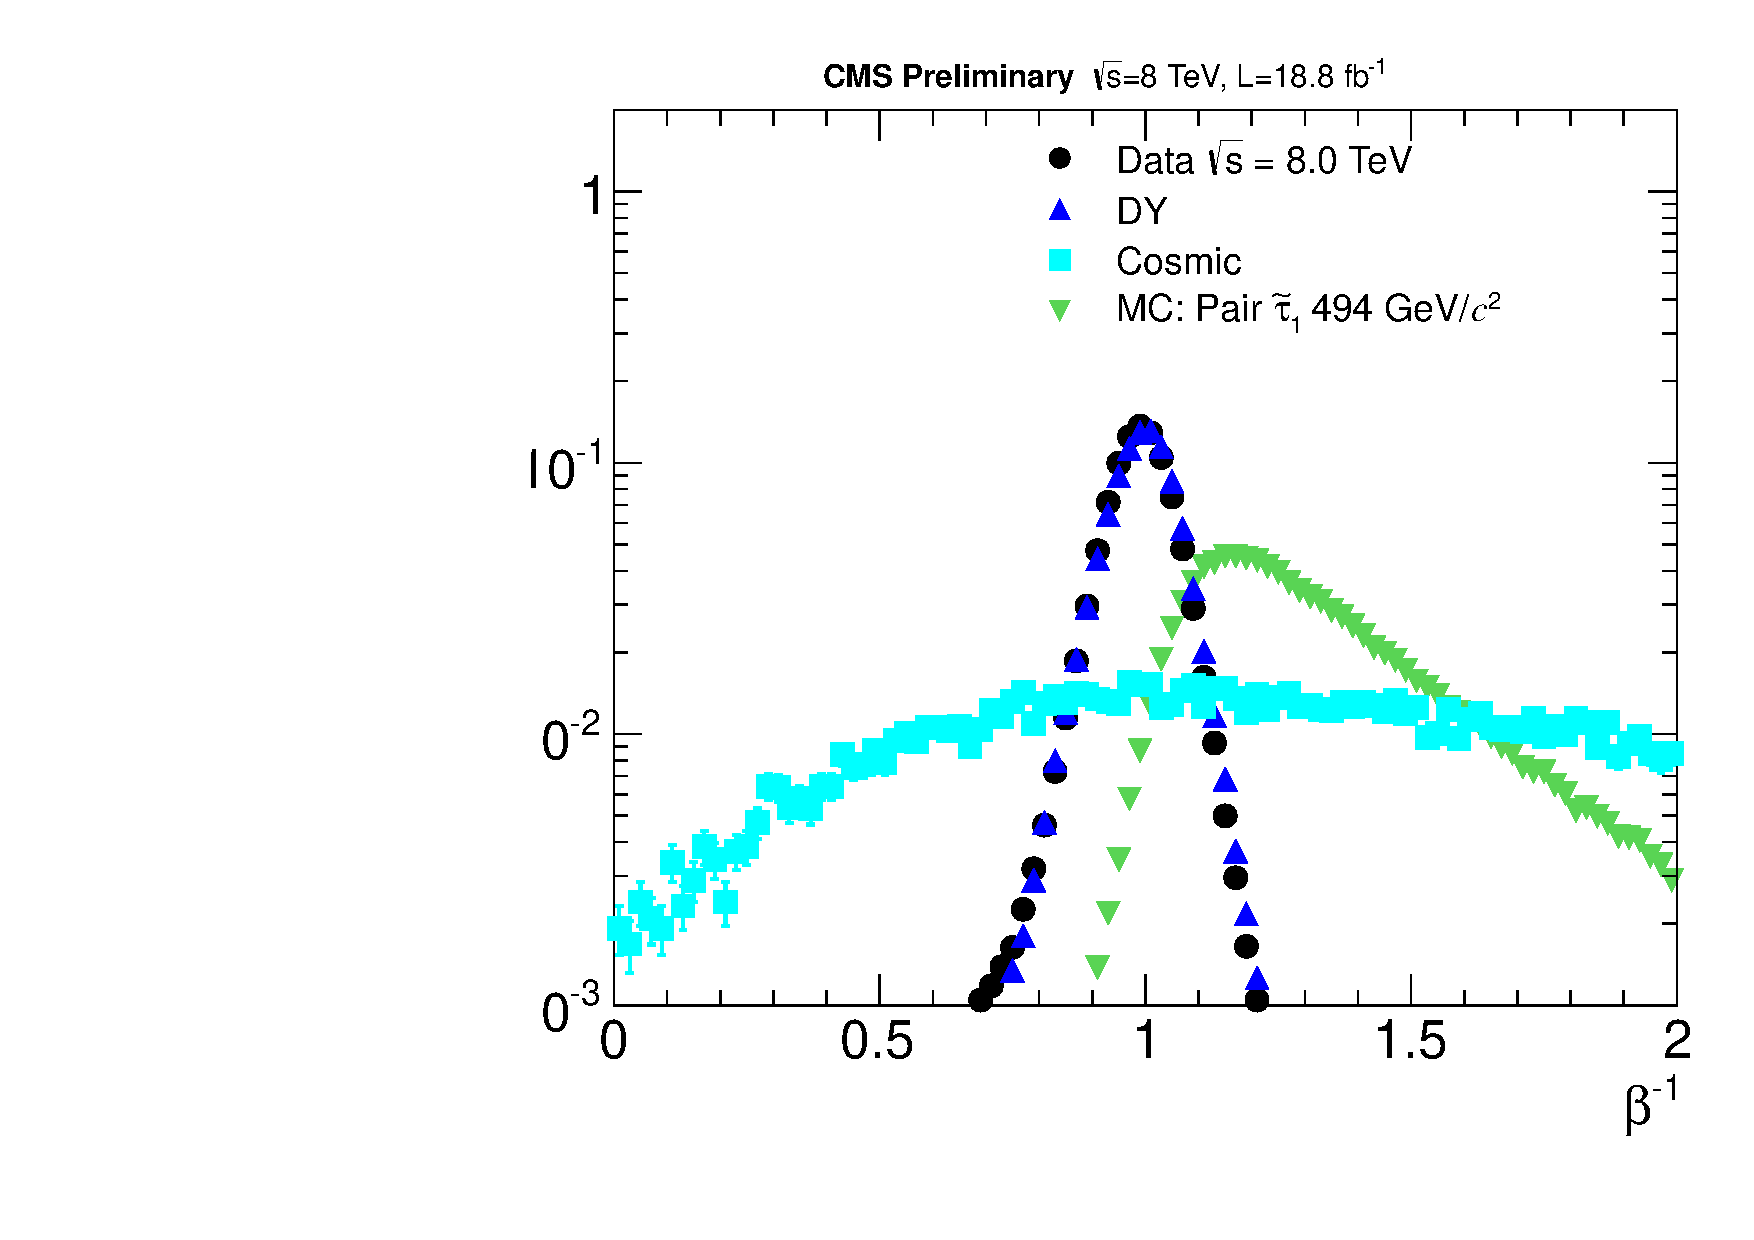
\includegraphics[width=0.49\textwidth]{figures/timing/TOF}
      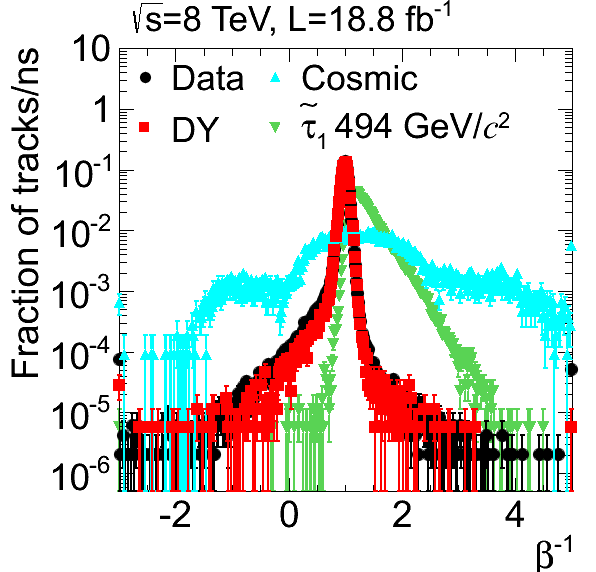
\includegraphics[width=0.49\textwidth]{figures/timing/TOFLog} \\
      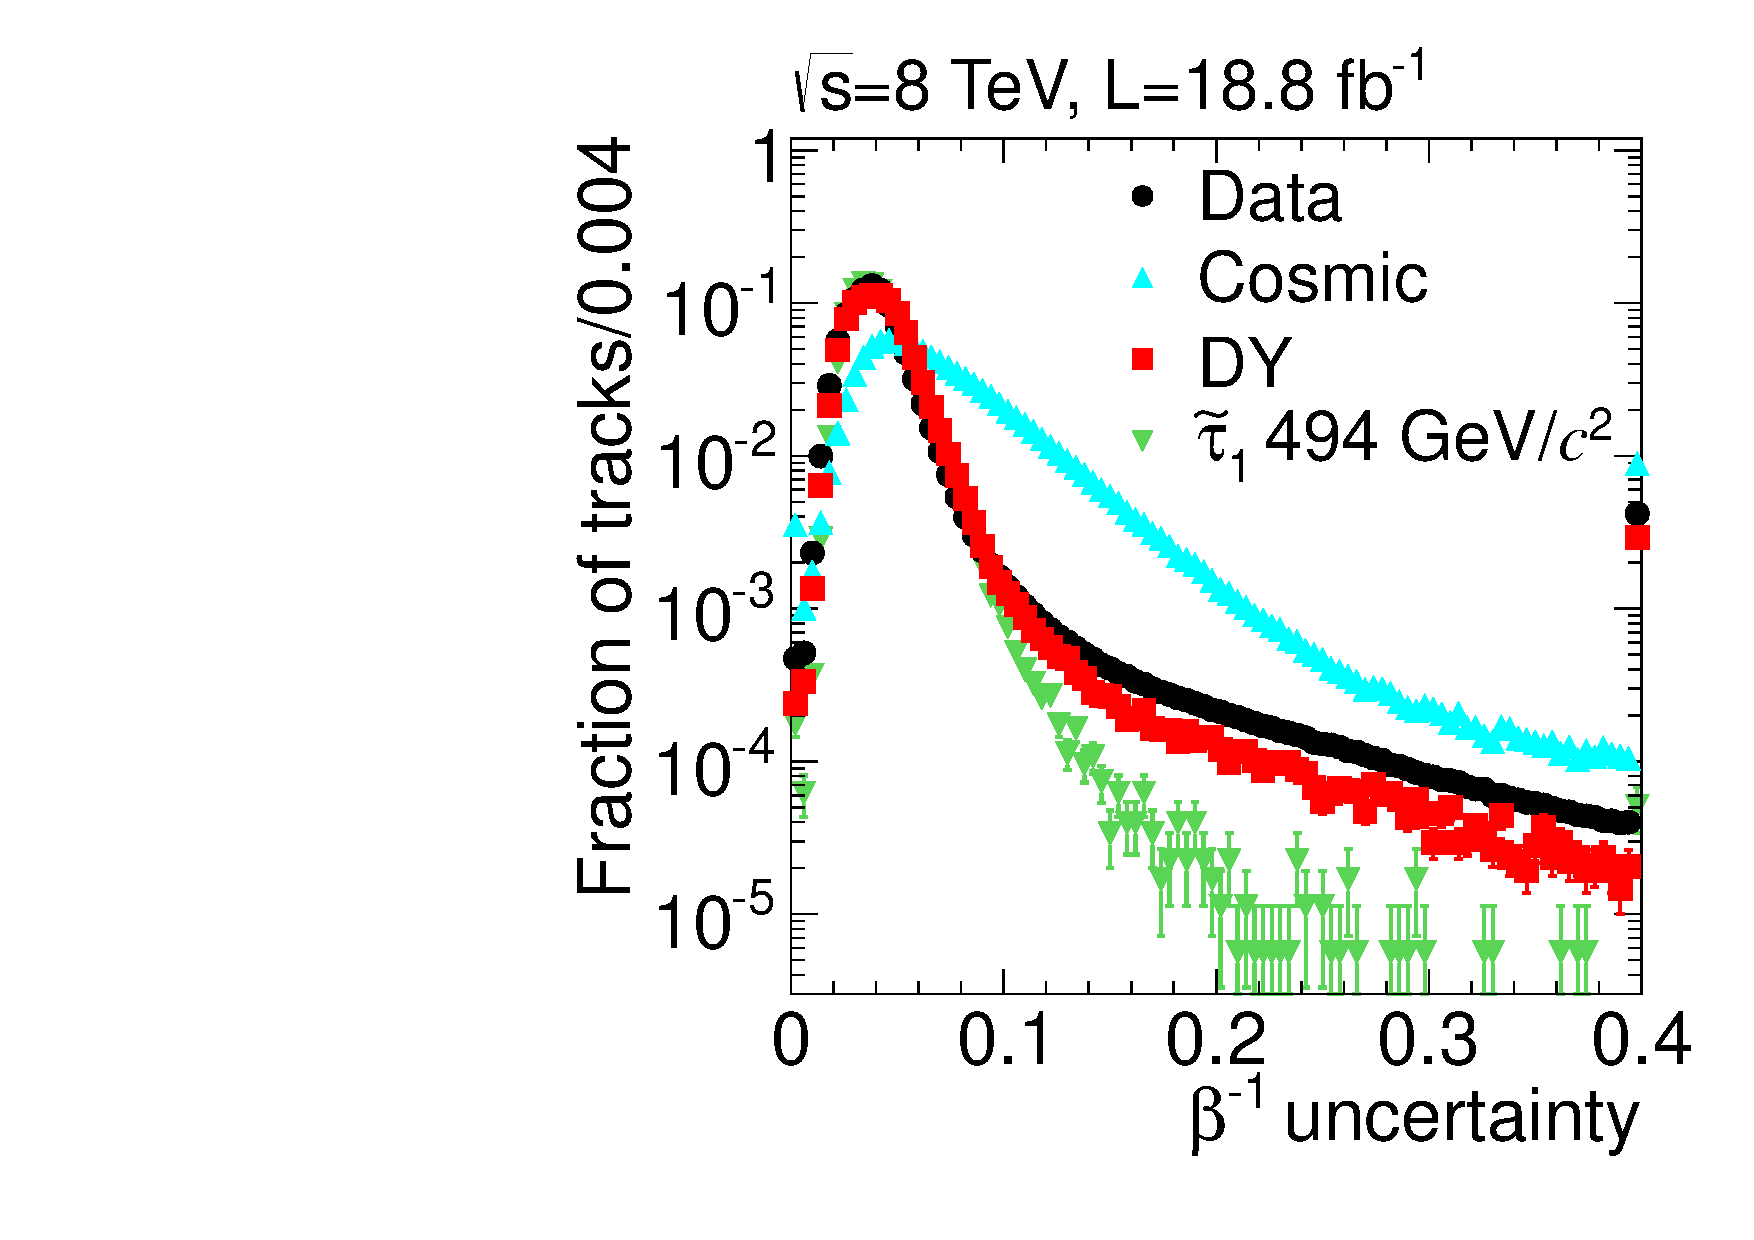
\includegraphics[width=0.49\textwidth]{figures/timing/TOFErr}
      \includegraphics[width=0.49\textwidth]{figures/timing/TOFNDof} \\
      \caption[Distribution of \invbeta\ and associated quantities]
      {Distribution of \invbeta\ and associated quantities for data,
simulated Drell-Yan production of photons and Z bosons decaying to muons (DY), muons from cosmic-rays, and simulated HSCPs.
The top row is the \invbeta\ measurement with linear y-axis scale (left) and log scale (right).
The bottom row is the uncertainty on the \invbeta\ measurement (left) and the number of degrees of freedom for the measurement (right).
For all plots the leftmost and rightmost bins contain the underflow and overflow, respectively.
        }
      \label{fig:invbeta}
  \end{center}
\end{figure}

The tails in the \invbeta\ distribution for collision muons can be greatly reduced by applying minimal quality requirements on the measurement.
This can be seen in Fig.~\ref{fig:invbetaQual} (top row) which shows the \invbeta\ distribution for the same
four samples after requiring the uncertainty on the \invbeta\ measurement
to be less than 0.07 and for the measurement to have at least eight degrees of freedom.

The average \invbeta\ value as a function of $\eta$ and \pt\ is shown in Fig.~\ref{fig:invbetaQual} (bottom row) for the same data sample described above
with the quality requirements on the \invbeta\ measurement applied.
The average can be seen to have small fluctuations versus $\eta$ over most of the $\eta$ range with a larger deviation at the most extreme $|\eta|$ values.
The average is almost completely flat against the reconstructed \pt\ of the muon.

\begin{figure}
  \begin{center}
      \includegraphics[width=0.49\textwidth]{figures/timing/TOFQual}
      \includegraphics[width=0.49\textwidth]{figures/timing/TOFQualLog} \\
      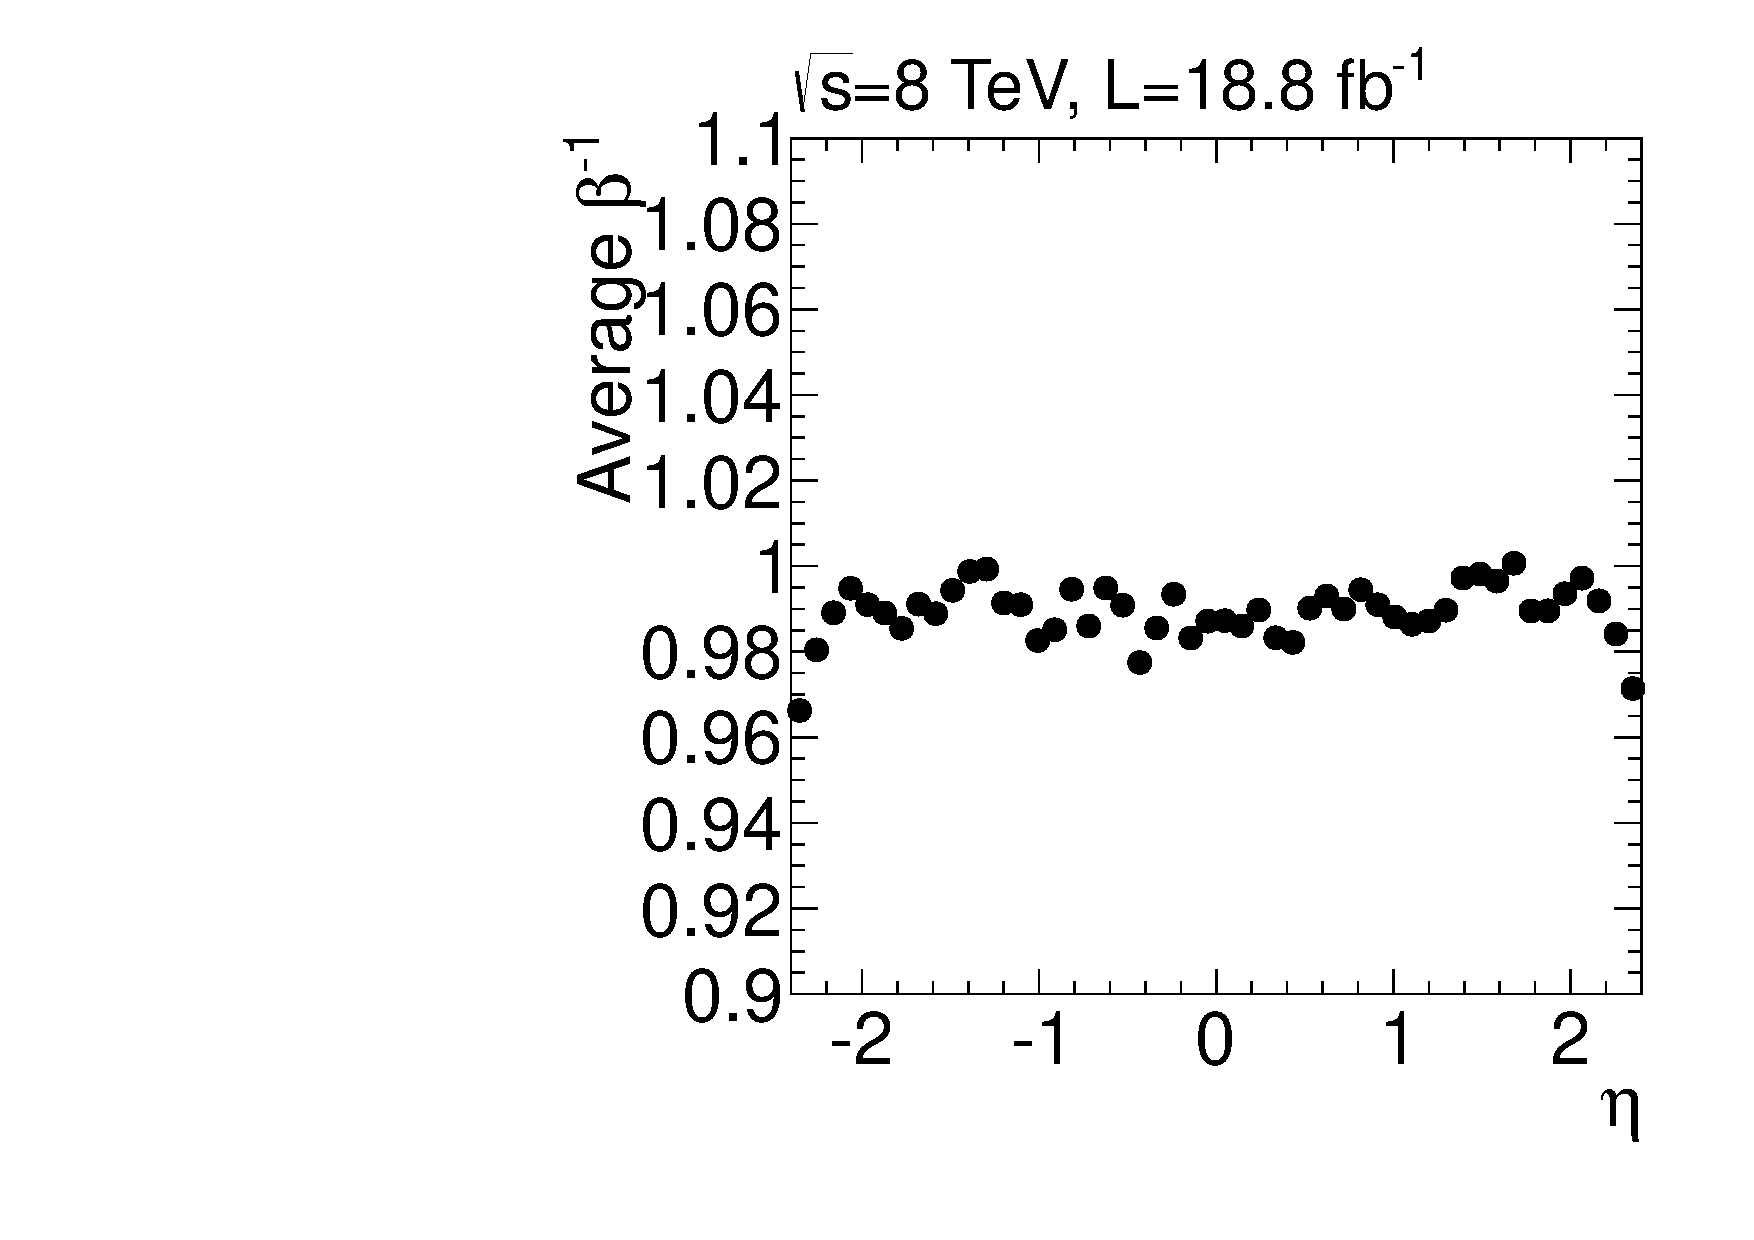
\includegraphics[width=0.49\textwidth]{figures/timing/TOFVsEta}
      \includegraphics[width=0.49\textwidth]{figures/timing/TOFVsPt} \\
      \caption[Distribution of \invbeta\ and associated quantities after applying quality requirements]
      {Distribution of \invbeta\ and associated quantities after applying quality requirements. 
The top row is the \invbeta\ measurement with linear y-axis scale (left) and log scale (right) for data,
simulated Drell-Yan production of photons and Z bosons decaying to muons (DY), muons from cosmic-rays, and simulated HSCPs.
Both plots have the underflow and overflow included in the leftmost and rightmost bins, respectively.
The bottom row is the average \invbeta\ measurement versus $\eta$ (left) and \pt\ (right).
        }
      \label{fig:invbetaQual}
  \end{center}
\end{figure}

The second variable, vertex time, is the estimated time the particle 
left the interaction point assuming it traveled at the speed of light.
This means setting \invbeta\ to one in Eq.~\ref{eq:speedred} reducing the equation to simply $t_0 = t$. 
For muons with at least a modest amount of $p_T$ that are produced in a collision in the triggered bunch crossing window this assumption is valid and thus the
value should be centered at zero. Figure~\ref{fig:vertextime} shows the vertex time, its uncertainty, and number of degrees of freedom
for the same four samples as in Fig.~\ref{fig:invbeta}. It can be seen that collision muons are tightly centered around zero while the cosmic-ray muons
are much more spread out Thus the timing measurement can be used to greatly reduce backgrounds from cosmic-ray muons. 

In future operation of the LHC, it is planned to have smaller spacing between proton bunches and more collisions per bunch crossing window.
This could potentially lead to muons from bunch crossings adjacent to the crossing triggered for readout being reconstructed in the event.
Timing in the muon system could be used to identify and remove these muons.

\begin{figure}
  \begin{center}
      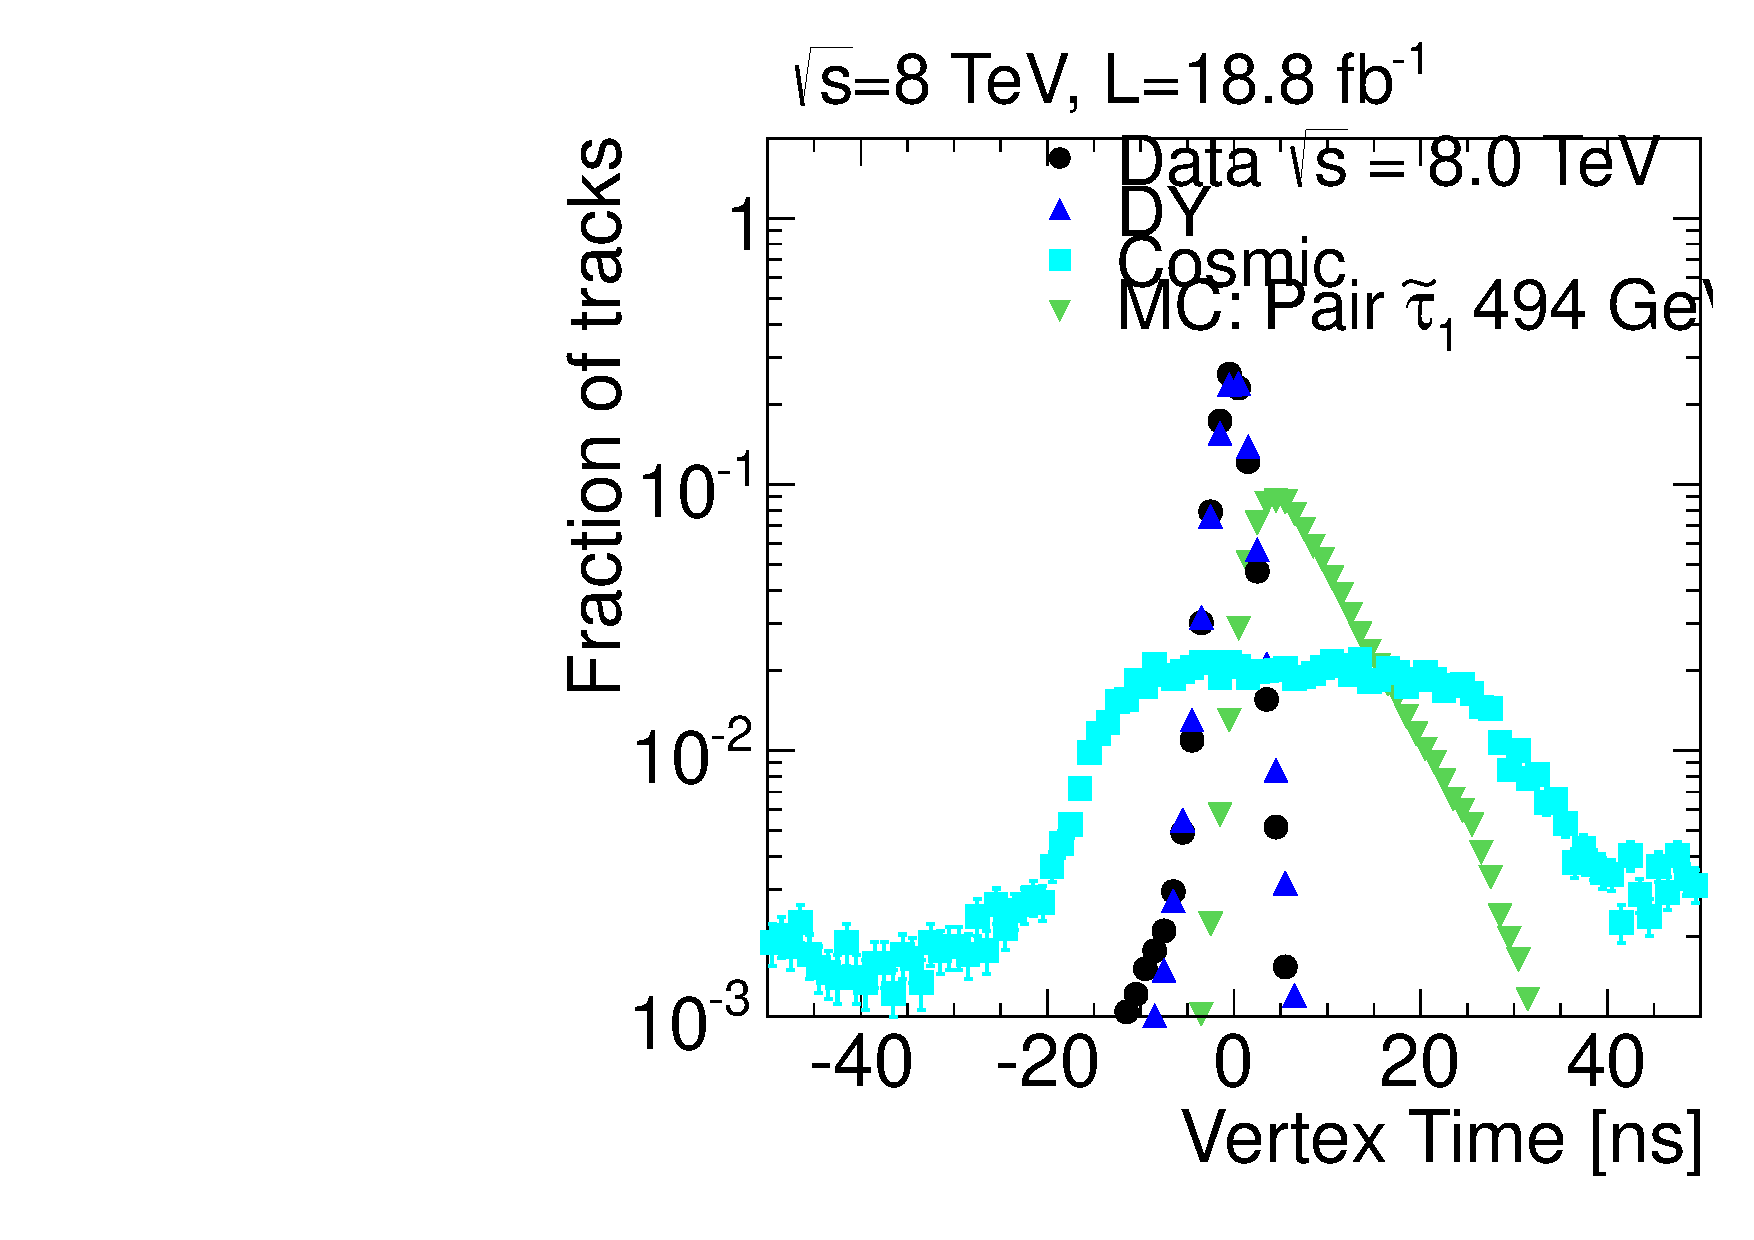
\includegraphics[width=0.49\textwidth]{figures/timing/Vertex}
      \includegraphics[width=0.49\textwidth]{figures/timing/VertexLog} \\
      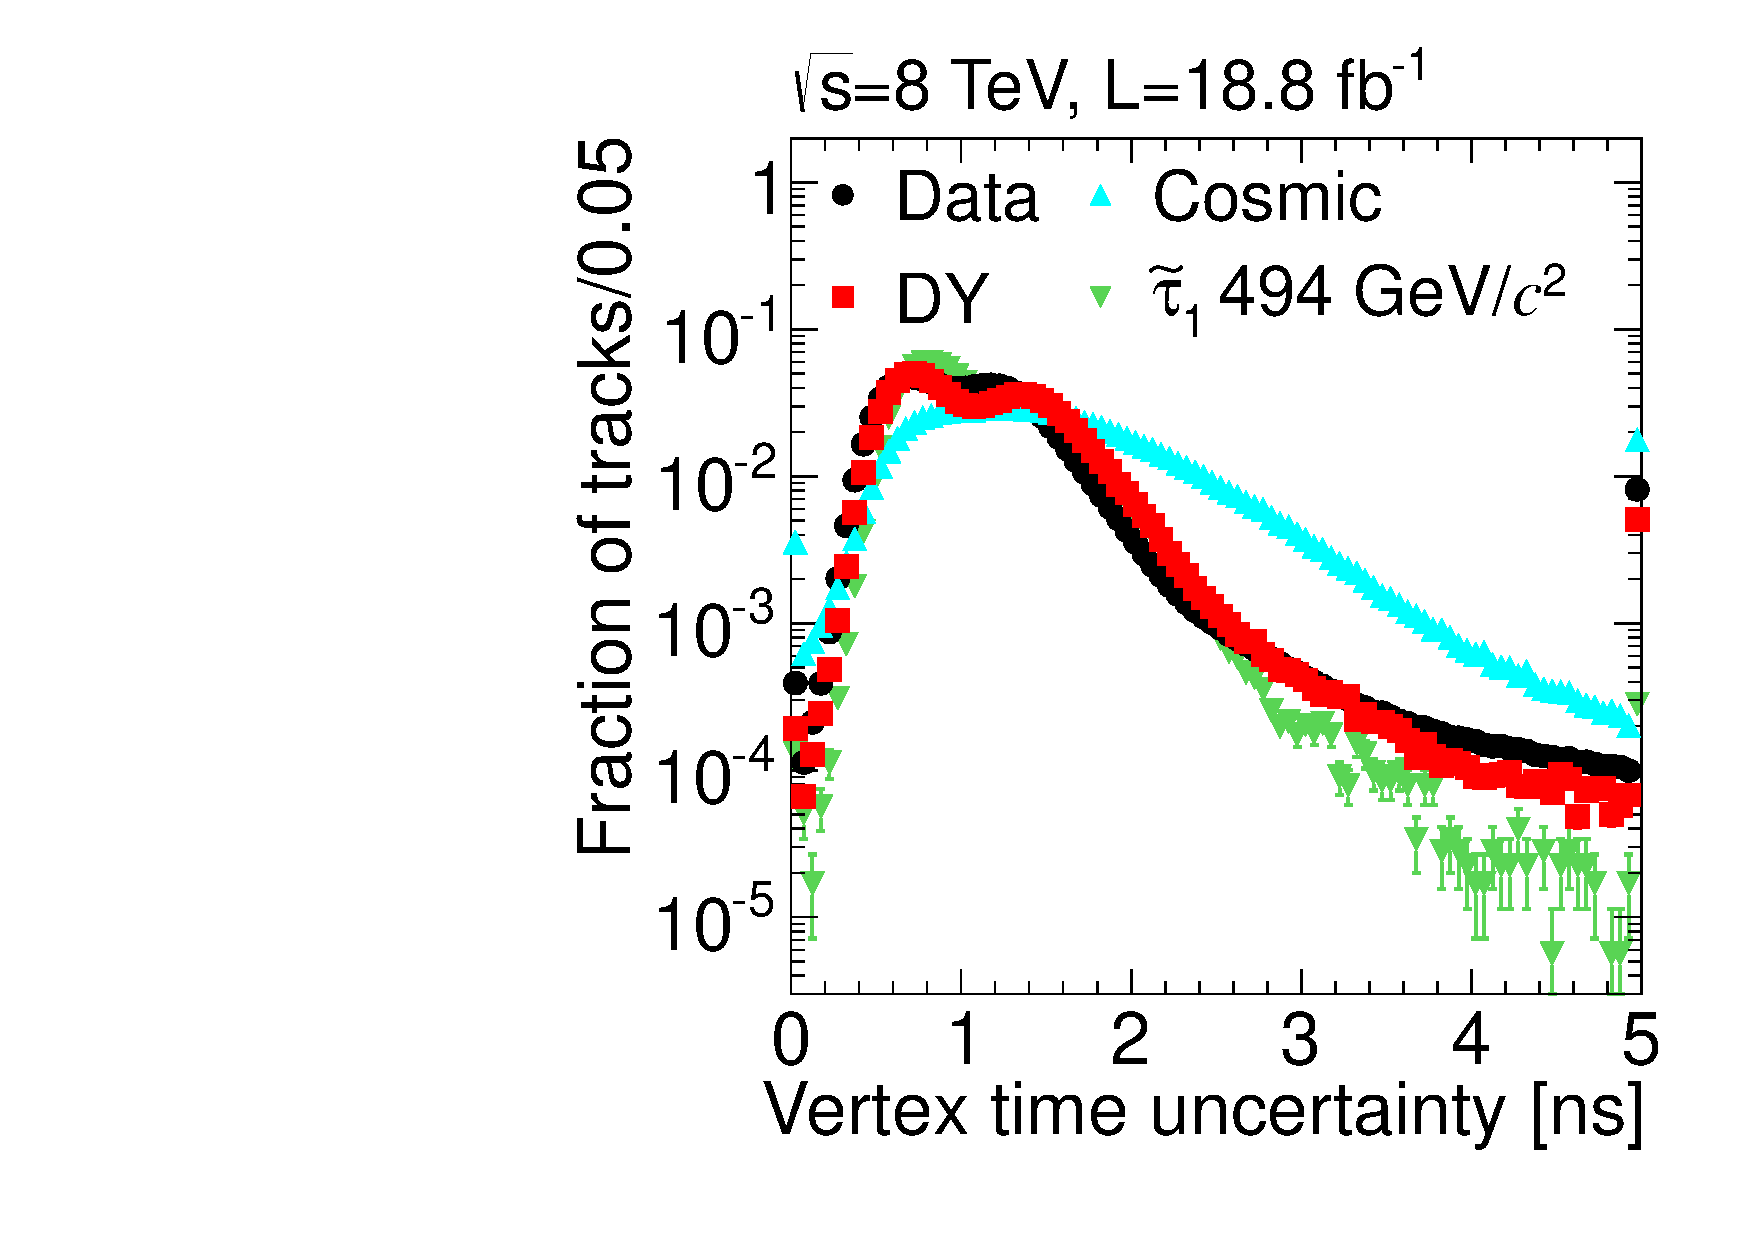
\includegraphics[width=0.49\textwidth]{figures/timing/VertexErr}
      \includegraphics[width=0.49\textwidth]{figures/timing/VertexNDof} \\
      \caption[Distribution of vertex time and associated quantities]
      {Distribution of vertex time and associated quantities for data,
simulated Drell-Yan production of photons and Z bosons decaying to muons (DY), muons from cosmic-rays, and simulated HSCPs.
The top row is the vertex time measurement with linear y-axis scale (left) and log scale (right).
The bottom row is the uncertainty on the vertex time measurement (left) and the number of degrees of freedom for the measurement (right).
For all plots the leftmost and rightmost bins contain the underflow and overflow, respectively.
        }
      \label{fig:vertextime}
  \end{center}
\end{figure}

%The last variable, time at vertex out in, is similar but it assumes the particle is traveling into CMS, such that the parameter $t_0$ represents the time an incoming particle
%would have crossed the interaction point. This can be an interesting property because tracks can be found in the inner tracker within a small time window so an incoming
%cosmic reconstructed in the inner tracker would likely have a $t_0$ from this measurement near zero. 
%The measurement assumes \invbeta\ = -1 reducing~\ref{eq:speed} to $t = -2 (d / c) + t_0$ which can be written to $t_0 = -2 (d / c) + t$ which makes it clear that
%$t_0$ can be found as the average of this quantity with weights like the previous measurement. Figure~\ref{fig:vertexopptime} shows the distribution of this time
%for the same three samples as above.

%\begin{figure}
%  \begin{center}
%      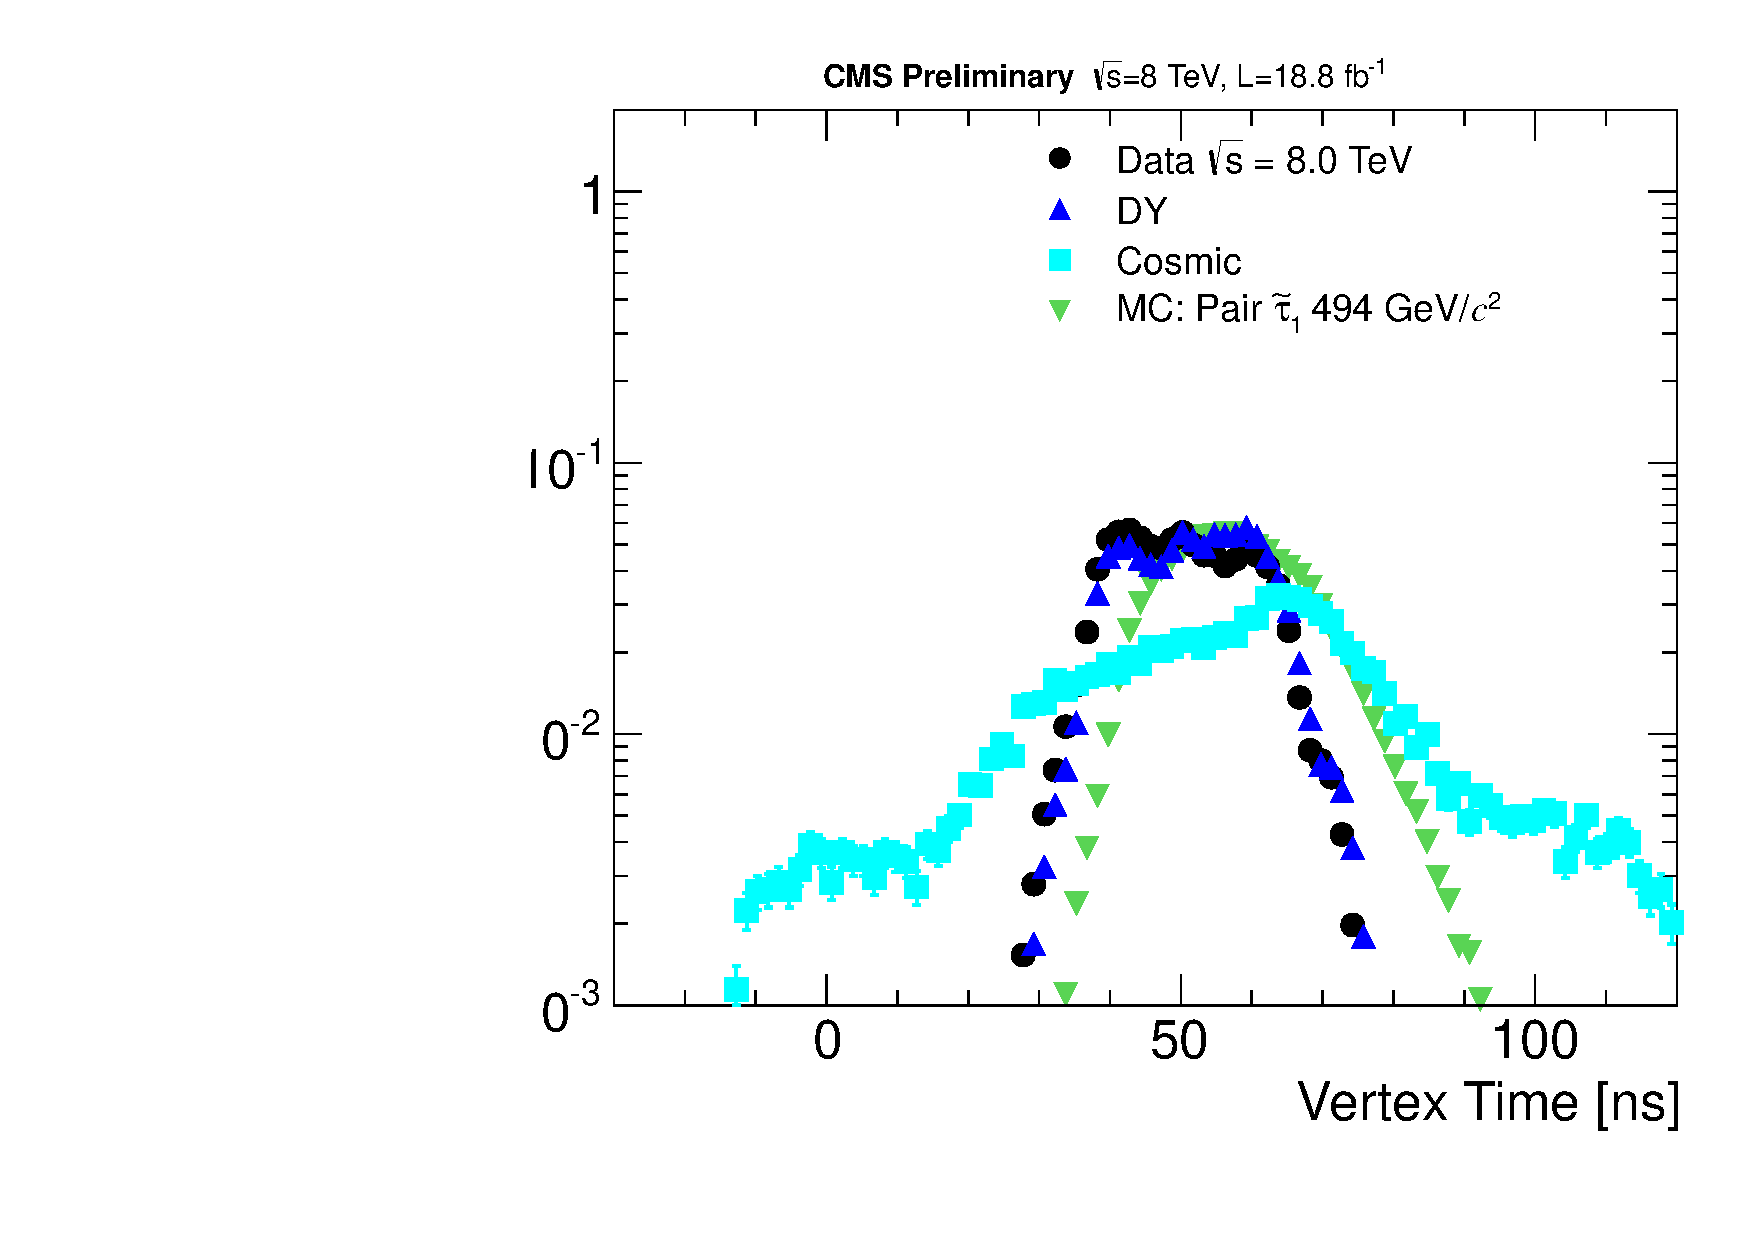
\includegraphics[width=0.44\textwidth]{figures/timing/VertexOpp}
%      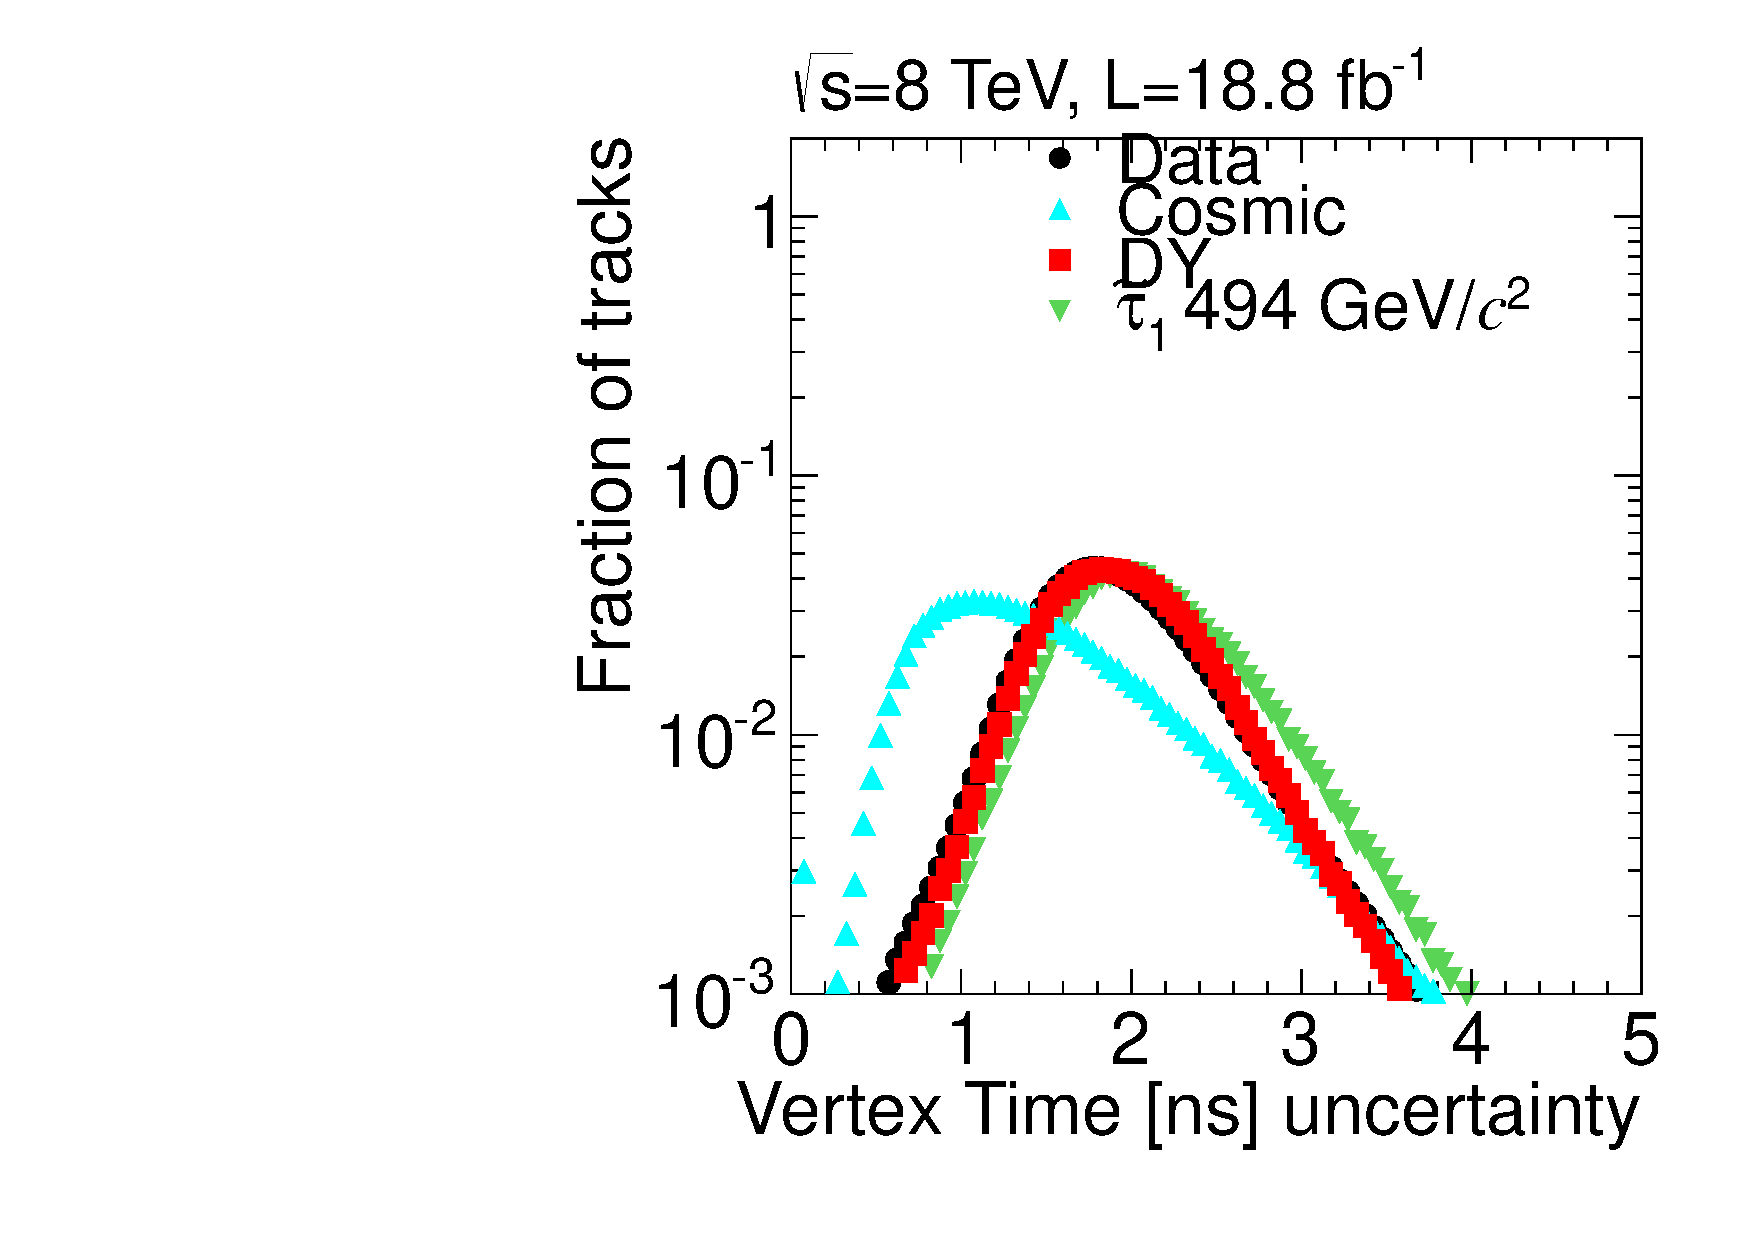
\includegraphics[width=0.44\textwidth]{figures/timing/VertexOppErr} \\
%      \caption[Distribution of time at vertex out in and the uncertainty on time at vertex out in]
%     {Distribution of time at vertex out in and the uncertainty on time at vertex out in for data,
%simulated Drell-Yan production of photons and Z boson decaying to muons (DY), muons from cosmic-rays, and simulated HSCPs
%}
%      \label{fig:vertexopptime}
%  \end{center}
%\end{figure}

The question may be asked why not to make a measurement without making any assumptions on $t_0$ or \invbeta. This was checked but it was found to have
resolution worse by more than an order of magnitude and very little discriminatory power.
This is because the assumptions in the previous measurements allowed both of them to use information
related to the beam spot, which is approximately three times as far away from the innermost part of the muon system as the outermost part is to the innermost part.
The vertex time measurement assumed an error-free propagation of the time in the muon system to the interaction point while the \invbeta\ measurement
added a new measurement at the interaction point with $t = 0$. This assumption-free measurement is not used for any purpose in CMS.

%\section{Timing in simulation} Maybe

%\section{Conclusion}
